\documentclass[]{fairmeta}

%\usepackage{amsmath,amsthm,amssymb,bm}
\usepackage{amsmath,amssymb,bm}
\usepackage[utf8]{inputenc}
\usepackage{caption}

\usepackage{color}
\usepackage{algorithm}
\usepackage[noend]{algpseudocode}
\usepackage[ruled,algo2e]{algorithm2e}%
\usepackage{derivative}
\usepackage{longtable}
\usepackage{pifont}
\usepackage{mdframed}
\usepackage{enumitem}
\usepackage{mathrsfs}
\usepackage{nicefrac}
\usepackage{subcaption}
\usepackage{float}
\newfloat{algorithm}{t}{lop}


\usepackage[normalem]{ulem}

\usepackage{siunitx}
\usepackage{tocloft}

\let\oldaddcontentsline\addcontentsline
\newcommand{\stoptocentries}{\renewcommand{\addcontentsline}[3]{}}
\newcommand{\starttocentries}{\let\addcontentsline\oldaddcontentsline}

\usepackage{tikz}
\usetikzlibrary{positioning, fit, calc}

\usepackage{booktabs}

\usepackage{arydshln} % Required for dashed lines
\usepackage{color}
\usepackage[table]{xcolor}
\usepackage{booktabs}
\usepackage{array}
\usepackage{colortbl}  % Added this package


\input{preamble}

% Shorthands for this project
\newcommand{\fX}{\bm{X}}
\usepackage{xspace}
\newcommand*{\eg}{{\it e.g.}\@\xspace}
\newcommand*{\ie}{{\it i.e.}\@\xspace}
\DeclarePairedDelimiterX{\infdivx}[2]{(}{)}{%
  #1\;\delimsize\|\;#2%
}
\newcommand{\infdiv}{D_\text{KL}\infdivx}
\newcommand*{\matr}[1]{\mathbfit{#1}}
\newcommand*{\tran}{^{\mkern-1.5mu\mathsf{T}}}

%\usepackage{xcolor} % Make sure you have this package!
\usepackage{graphicx}
\usepackage[most]{tcolorbox}

\definecolor{mygray}{gray}{0.95}
\newcommand{\graybox}[1]{%
\vspace{-1em} 
\begin{center}			% Centering minipage
\colorbox{mygray} {		% Set's the color of minipage
\begin{minipage}{0.987\linewidth} 	% Starts minipage
\centering
\vspace{-1em}   
{#1}    
\end{minipage}}			% End minipage
\end{center}
}

% Define colors
\definecolor{salmon}{RGB}{250,128,114}
\definecolor{cornflowerblue}{RGB}{100,149,237}


% \theoremstyle{definition}
% \newtheorem{definition}{Definition}[section]

\title{Aligning Protein Language Models with Large-Scale Mutant Preferences}

\author[1]{Nikša Praljak}

\affiliation[1]{University of Chicago}

\abstract{
Protein language models (pLMs) have demonstrated remarkable capabilities in structure prediction with clear scaling laws as model size increases. However, despite their success in protein structure tasks, pLMs show limited performance in predicting mutation effects, with capabilities that often plateau or decline with increased model size. We present StableESM, a stability-aligned protein language model created by applying Direct Preference Optimization (DPO) to ESM2 using large-scale experimental stability data comprising up to 1 million mutations across approximately 1000 different protein domains from MegaScale, Human Domainome 1, and FireProtDB. Similar to the transition from GPT-3 to ChatGPT through reinforcement learning from human feedback, we investigate whether learning from mutation preferences can unlock scaling laws in pLMs for mutation effect prediction while enabling the model to learn features and capabilities that generalize to completely unseen proteins and their mutation effects. Our results demonstrate that larger pLMs show enhanced capability in improving mutation effect prediction during preference optimization, with benefits generalizing to unseen protein homologs and families. Notably, StableESM exhibits improved zero-shot mutation effect prediction, accurately assessing stability changes in proteins never encountered during training and improving predictions on unseen tasks like double mutation effects and disorder region prediction. Importantly, StableESM avoids catastrophic forgetting, maintaining or improving performance on structure prediction and other protein modeling tasks compared to the base ESM2 model. As a practical application of our approach, we demonstrate the design of thermostable multicopper oxidase variants using a machine learning-directed evolution approach to improve catalytic activity at high temperatures, identifying beneficial mutations that would be missed by unaligned models. This work presents a comprehensive computational and experimental investigation of aligning protein language models with experimental preferences, systematically probing the effectiveness and utility of this approach for enhancing mutation effect prediction while maintaining performance on foundational protein modeling tasks.
}

\stoptocentries

% \date{\today}
\correspondence{Nikša Praljak at \email{niksapraljak1@uchicago.edu}}

% \metadata[Code]{\url{TBD}}




\begin{document}

\maketitle

\section{Introduction}
\label{sec:intro}

Large-scale pretraining has ushered in a new renaissance in computational sciences, demonstrating that model performance scales predictably with increased parameters and training data~\citep{kaplan2020scaling,hoffmann2022training}. This scaling paradigm has enabled remarkable capabilities in language models, from GPT-3's few-shot learning to sophisticated reasoning abilities that emerge at sufficient scale~\citep{brown2020language}. Similarly, protein language models (pLMs) trained on millions of protein sequences using self-supervised learning techniques have demonstrated clear scaling laws for structure prediction and contact prediction tasks, with larger models consistently outperforming smaller counterparts~\citep{rives2021biological,lin2023evolutionary}.

However, scaling alone has revealed fundamental limitations in both domains. Despite impressive capabilities on many tasks, large language models trained purely on next-token prediction often fail to align with human intentions, generating outputs that can be unsafe, biased, or unhelpful~\citep{ouyang2022training}. Remarkably, protein language models exhibit a parallel phenomenon: while larger models excel at structure-related tasks, their zero-shot mutation effect prediction performance saturates or even deteriorates with increased model size, suggesting that raw scaling is insufficient for capturing the nuanced relationship between sequence changes and functional outcomes~\citep{meier2021language,gordon2024protein,li2024feature,hou2025understanding}. Recent work suggests this scaling failure occurs because oversized models overfit to phylogenetic noise rather than functional constraints~\citep{weinstein2022non}, which may indicate that post-training alignment with experimental data could provide a path to redirect models away from evolutionary confounds toward biologically relevant fitness landscapes.

This saturation in mutation effect prediction performance with increased model size has prompted investigation into alternative approaches for improvement. While some studies have demonstrated that incorporating curated multiple sequence alignments (MSAs) or structural context through deep learning architectures can enhance mutational effect prediction~\citep{notin2022tranception,paul2023combining}, remarkably, simple baseline methods using only evolutionary conservation scores and basic structural features like solvent accessibility often achieve comparable performance to state-of-the-art large protein language models~\citep{tsishyn2025residue}. This striking observation raises fundamental questions about what representations these billion-parameter models are actually learning for mutation effect prediction and whether their impressive parameter counts are effectively utilized for this critical task. The fact that simple heuristics can match sophisticated language models suggests that current pretraining objectives may not be optimally aligned with the goal of understanding mutational consequences, pointing toward the need for targeted post-training optimization approaches that can unlock the latent capabilities of large protein language models for mutation effect prediction.

Accurate mutation effect prediction is critical not only for practical applications in drug design and enzyme engineering~\citep{arnold2017directed,romero2009exploring}, but also for understanding the clinical impact of single mutations in human diseases~\citep{frazer2021disease,cheng2023accurate}, and represents a fundamental requirement for ideal protein models. To understand how proteins traverse adaptive landscapes through evolution, we must first accurately predict individual mutational effects—only then can we model how evolution explores local sequence landscapes to acquire new functions through incremental changes that maintain protein function (i.e., Maynard Smith paths)~\citep{maynard1970natural,weinreich2006darwinian}, with co-evolving networks of residues constraining viable evolutionary trajectories~\citep{halabi2009protein}. Thus, our models should aim to perfectly predict these fitness landscapes to truly understand how proteins evolve and function.

The transformation from GPT-3 to ChatGPT demonstrated that post-training alignment using reinforcement learning from human feedback (RLHF) could unlock model capabilities while ensuring safer, more helpful behavior~\citep{ouyang2022training}. This breakthrough required only tens of thousands of human preference judgments—a remarkably small dataset compared to the trillions of tokens used in pretraining—yet fundamentally altered model behavior through techniques like proximal policy optimization~\citep{schulman2017proximal} and direct preference optimization~\citep{rafailov2023direct,lambert2024tulu}.

The explosive growth of experimentally validated protein variants across diverse protein families~\citep{fowler2014deep,fowler2023atlas} suggests that protein language models may be poised for a similar alignment breakthrough. Large-scale mutagenesis studies now provide millions of experimental measurements linking sequence changes to functional outcomes, creating an unprecedented opportunity to apply post-training optimization techniques to protein design. Unlike fitness or activity measurements that may be beneficial in one context while deleterious in another, protein stability represents a relatively context-agnostic property that can be assessed through zero-shot log-likelihood ratios, making it an ideal target for large-scale alignment efforts.

Recent efforts have begun applying reinforcement learning and post-training techniques to protein language models. ProteinDPO used direct preference optimization to improve ESM-IF's thermostability predictions~\citep{widatalla2024aligning}; RLXF applied proximal policy optimization with experimental feedback to ESM2 for fluorescent protein design~\citep{blalock2025functional}; ProtRL provided a general RL framework for steering autoregressive models like ZymCTRL toward specific design objectives~\citep{stocco2024guiding}; ProteinRL, LatProtRL, and RL-DIF explored various architectures and reward formulations~\citep{sternke2023proteinrl,lee2024robust,ektefaie2024reinforcement}; and ProGen3 used iterative reasoning preference optimization (IRPO) on fitness data to achieve impressive gains across model scales, with larger models benefiting more from alignment~\citep{bhatnagar2025scaling,pang2024iterative}. While these pioneering studies demonstrated the promise of post-training alignment, with ProGen3 notably showing that preference-based alignment prevents performance saturation in larger models, they have been limited by focus on generation tasks, specific protein families, or lack of comprehensive evaluation across diverse benchmarks. Our work explores complementary aspects: we apply Direct Preference Optimization to learn from $\sim$1 million relative mutation preferences across approximately 1,000 protein domains (combining MegaScale~\citep{tsuboyama2023mega}, Human Domainome 1~\citep{beltran2025site}, and FireProtDB~\citep{stourac2021fireprotdb}), focus specifically on stability as a universal alignment signal that enables zero-shot mutation effect prediction, demonstrate generalization to completely unseen protein families and transfer to unrelated tasks (disorder prediction, double mutations), comprehensively evaluate catastrophic forgetting across structure prediction and clinical variant assessment, and provide experimental validation of thermostable enzyme variants that would be missed by unaligned models.

Here, we present StableESM, a stability-aligned protein language model created by applying Direct Preference Optimization to ESM2 models ranging from 8M to 3B parameters using experimental stability data comprising approximately 1 million mutations across 1,000 protein domains from MegaScale, Human Domainome 1, and FireProtDB. Our results demonstrate that alignment through experimental preferences not only enhances mutation effect prediction capabilities regardless of base model size but addresses each of the critical limitations in current protein language model alignment approaches. StableESM exhibits improved zero-shot generalization to completely unseen protein homologs and families, improves performance on tasks unrelated to the stability alignment objective including double mutation effects and disorder region prediction, avoids catastrophic forgetting across diverse protein modeling tasks from structure prediction to clinical variant assessment, and enables experimental discovery of thermostable multicopper oxidase design alleles and variants that would be missed by unaligned models. Most importantly, we show that larger protein language models exhibit enhanced capability for improvement during preference optimization, establishing a new paradigm for comprehensively aligning protein language models with experimental data to enhance their predictive capabilities while maintaining their foundational knowledge.


\section{Results}\label{sec:prelim_generative_models}

\subsection{Large-scale modeling of mutational preferences using protein language models and Direct Preference Optimization}

Inspired by the success of aligning large language models with human preferences through techniques like RLHF, we developed an analogous framework for protein language models using experimental mutation data (Figure~\ref{fig:intro_stableESM}a). While language models learn to distinguish between preferred and non-preferred responses to human prompts, our approach trains protein language models to distinguish between experimentally validated stable and unstable protein variants (Figure~\ref{fig:intro_stableESM}b). This paradigm shift enables us to leverage the growing wealth of experimental mutagenesis data to directly optimize models for mutation effect prediction.

We curated a comprehensive preference dataset by combining three major experimental databases: MegaScale, Human Domainome 1, and FireProtDB (Figure~\ref{fig:intro_stableESM}c). Our curation process yielded approximately 1 million mutations across 1,154 unique protein domains, resulting in 143,578,400 preference pairs for training and 1,824,750 for validation (Methods \ref{sec:dataset_curation}). Each preference pair consists of two mutations from the same protein domain where one mutation is experimentally more stable than the other, providing a direct ranking signal for optimization.
The scale and diversity of this dataset represents a significant advance over previous protein alignment efforts. [Extended Figure X] demonstrates that our preference dataset spans a broad range of protein domain lengths (median: X residues), encompasses diverse sequence space as measured by ESM2 embeddings, and covers all major amino acid substitution types with balanced representation across stability categories. Notably, the dataset includes an average of X preference pairs per domain, ensuring sufficient signal for robust alignment across protein families.

We implemented StableESM using Low-Rank Adaptation (LoRA) applied to the pretrained ESM2 models, enabling efficient fine-tuning while preserving the original model weights (Methods \ref{sec:stableesm_implementation}). This approach allows us to adapt models across multiple scales (8M to 3B parameters) for preference optimization without the computational cost of full fine-tuning, while maintaining the rich evolutionary representations learned during pretraining. We applied Direct Preference Optimization (DPO) to train StableESM models, fundamentally shifting the training objective from masked language modeling to preference-based optimization (Figure~\ref{fig:intro_stableESM}d), Methods \ref{sec:dpo_training}). Unlike the vanilla ESM2 models trained to predict masked amino acids from evolutionary sequences, StableESM models learn to assign higher likelihood to experimentally stable mutations compared to unstable ones from the same protein context.

\begin{tcolorbox}[
  title=StableESM: Direct Preference Optimization Loss,
  colback=white,
  colframe=black!50,
  coltitle=black,
  colbacktitle=black!10,
  fonttitle=\bfseries
]
Our approach leverages log-likelihood ratios computed by masking mutation positions and calculating $\pi(y \mid x) = \frac{p(x_i = \text{mut} \mid x_{\setminus i})}{p(x_i = \text{wt} \mid x_{\setminus i})}$, where $x_{\setminus i}$ represents the sequence with position $i$ masked. Each preference pair consists of stable ($y_w$) and unstable ($y_l$) mutations from the same protein domain, but not necessarily the same sequence position. The DPO objective shifts training from masked language modeling to preference-based optimization:
\begin{equation}
\mathcal{L}_{\text{DPO}} = -\mathbb{E}_{(x, y_w, y_l) \sim \mathcal{D}} \left[ \log \sigma \left( \beta \log \frac{\pi_\theta(y_w \mid x)}{\pi_{\text{ref}}(y_w \mid x)} - \beta \log \frac{\pi_\theta(y_l \mid x)}{\pi_{\text{ref}}(y_l \mid x)} \right) \right]
\end{equation}
where $\pi_{\text{ref}}$ is the frozen ESM2 reference model, $\pi_\theta$ is the aligned model's log-likelihood ratios computed via the masking procedure, and $\beta$ controls the KL divergence constraint against the reference model (Methods~\ref{sec:stableesm_implementation},~\ref{sec:dpo_training}).
\end{tcolorbox}

The experimental preference signal provides a more direct supervision than evolutionary data alone, potentially enabling models to overcome the phylogenetic noise limitations identified in previous scaling studies. By training across model sizes from 8M to 3B parameters using identical preference datasets and optimization procedures, we can systematically investigate whether preference alignment unlocks improved scaling laws for mutation effect prediction in protein language models.


\begin{figure}[H]
    \centering
    \includegraphics[width=\textwidth]{figures/Figure_1.png}
    \caption{\textbf{StableESM: Aligning protein language models with experimental stability preferences using Direct Preference Optimization.} \textbf{(a)} Conceptual framework adapting preference-based alignment from large language models to protein language models. While language models learn to distinguish preferred from non-preferred responses to human prompts, protein language models can learn to distinguish experimentally stable from unstable protein variants. \textbf{(b)} Mutational protein preference learning paradigm. Given protein sequences with single mutations, StableESM learns to assign higher likelihood to experimentally stable mutations compared to unstable mutations from the same protein domain. \textbf{(c)} Large-scale preference dataset curation combining MegaScale, Human Domainome 1, and FireProtDB databases. The curated dataset contains approximately 1 million mutations across 1,154 protein domains, yielding 143,578,400 preference pairs for training and 1,824,750 for validation. Only single mutations are included in the preference dataset. \textbf{(d)} Training paradigm comparison between vanilla ESM2 and StableESM. ESM2 models are pretrained on evolutionary sequences using masked language modeling, while StableESM models undergo additional Direct Preference Optimization training to predict stable over unstable mutations using experimental preference data.}
    \label{fig:intro_stableESM}
\end{figure}

\subsection{Training StableESM on $\sim$1M experimental variants with Direct Preference Optimization}

We applied Direct Preference Optimization to ESM2 models across multiple scales (8M to 3B parameters) using our curated stability preference dataset. The DPO training objective successfully learned to distinguish between stable and unstable mutations, as evidenced by the convergence of training and validation losses (Figure~\ref{fig:train_eval_stableesm}a). The probability that stable mutations are preferred over unstable ones increased from the random baseline of 0.5 to approximately 0.70 during training, while both training and validation losses decreased smoothly without overfitting.

Importantly, our validation set represents a stringent test of generalization: while the protein domains are the same as those in the training set, the specific mutations are completely held out during training. This setup tests the model's ability to learn general principles of mutation effects within each protein context rather than memorizing specific mutation-stability relationships. The alignment between training and validation loss trajectories demonstrates that models are successfully learning transferable preferences that generalize to unseen mutations within the same protein domains.
The DPO loss curves demonstrate that the preference learning mechanism is working as intended across model sizes. Notably, the probability curves show that models consistently learn to assign higher likelihood to experimentally stable mutations compared to unstable ones from the same protein context, even for mutations never encountered during training.

[Extended Figure X] shows that this preference learning translates to improved mutation effect prediction performance on both training and validation splits, with Spearman correlations increasing substantially compared to vanilla ESM2 baselines. When evaluated on overlapping proteins from the ProteinGym benchmark suite, StableESM models achieve competitive performance despite being trained on preference ranking rather than direct regression of experimental values, demonstrating that the preference signal effectively captures mutation effect relationships.


\begin{figure}[H]
    \centering
    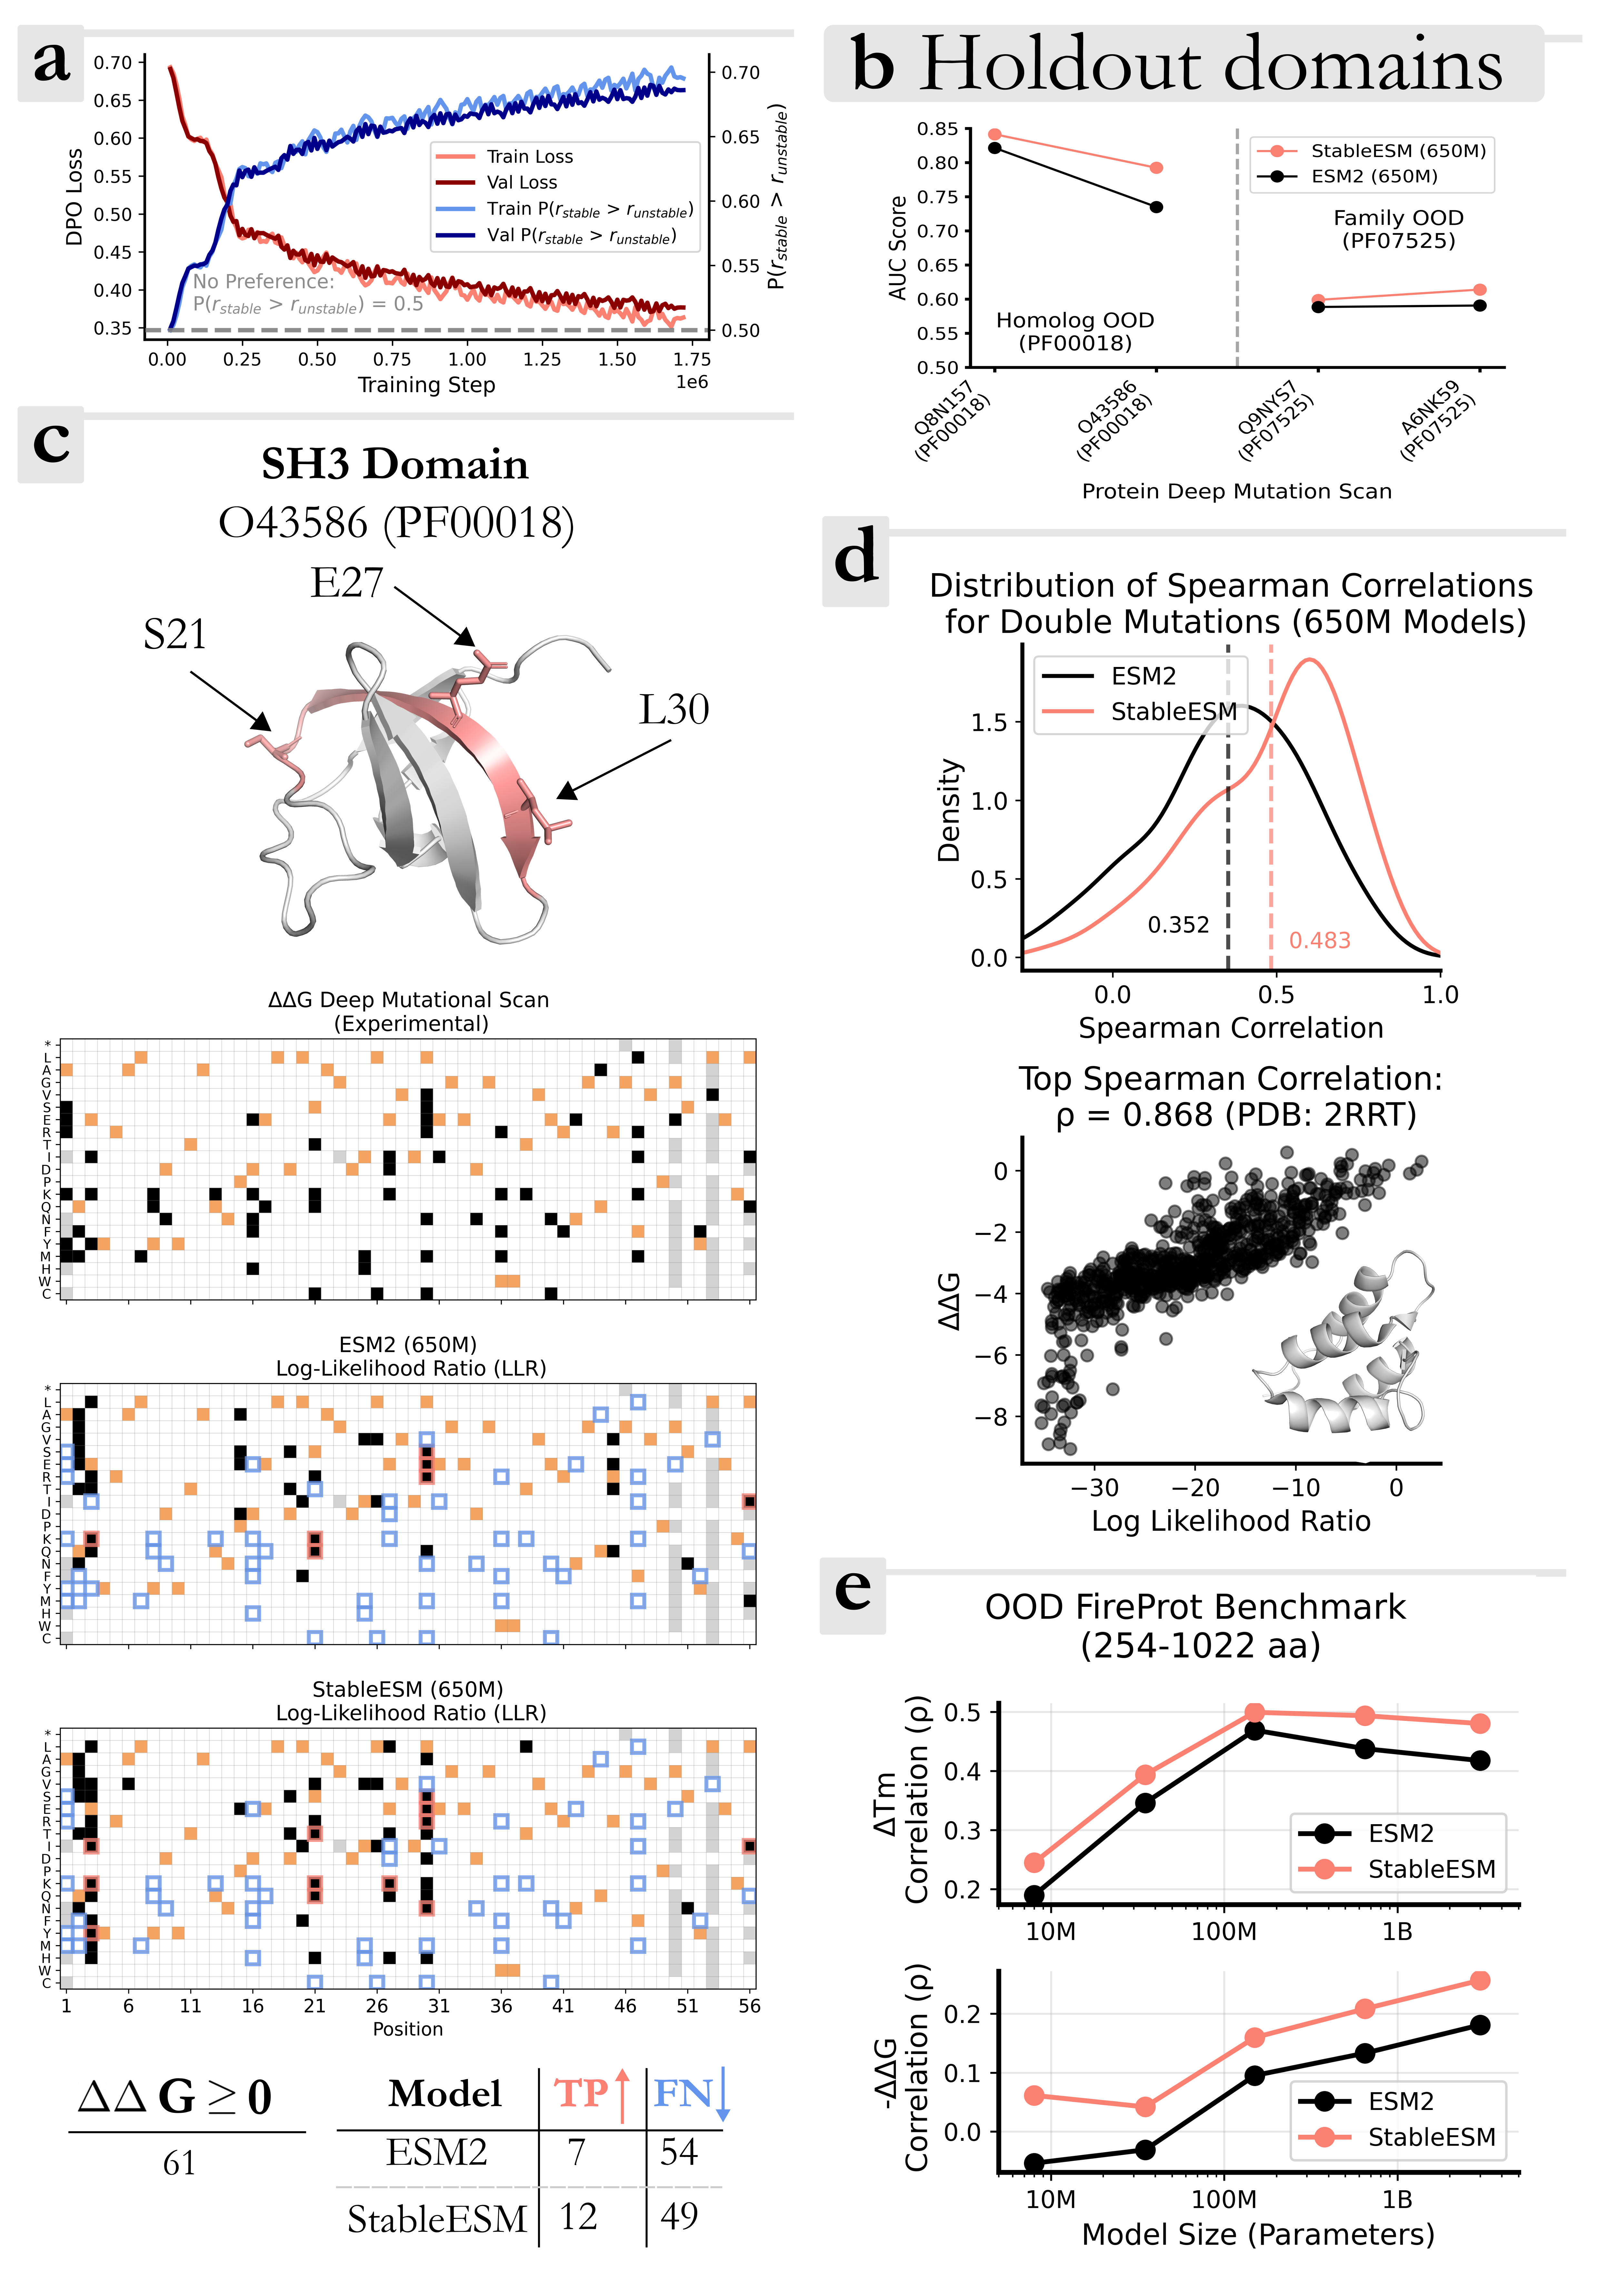
\includegraphics[width=\textwidth]{figures/Figure_2.png}
%    \label{fig:train_eval_stableesm}
\end{figure}

\captionof{figure}{\textbf{StableESM training dynamics and performance validation across scales and protein families.} \textbf{(a)} Direct Preference Optimization training curves for StableESM (650M parameters). Training and validation losses decrease smoothly while the probability of preferring stable over unstable mutations increases from random baseline (0.5) to $\sim$0.70, demonstrating successful preference learning without overfitting. \textbf{(b)} Zero-shot generalization to completely held-out protein domains across different protein families. StableESM (red) consistently outperforms ESM2 (black) on unseen protein domains, including challenging targets like homolog out-of-distribution (OOD) and family OOD evaluations. Dashed line indicates random performance. \textbf{(c)} Detailed mutation effect prediction for SH3 domain (O43586, PF00018). Top: Protein structure with highlighted residues corresponding to mutations. Middle: Experimental $\Delta\Delta G$ values compared to ESM2 and StableESM log-likelihood ratio predictions. Bottom: Correlation analysis showing StableESM achieves superior agreement with experimental measurements ($\rho$ = 0.483) compared to ESM2 ($\rho$ = 0.352). Best correlation achieved on PDB structure 2RRT ($\rho$ = 0.868). \textbf{(d)} Distribution of Spearman correlations for double mutation effect prediction across protein domains. StableESM (red) shows improved performance compared to ESM2 (black) for predicting higher-order mutational effects, with median correlation increasing substantially. \textbf{(e)} Scaling behavior for mutation effect prediction on OOD FireProt benchmark (254-1022 amino acids). Both $\Delta T_m$ (top) and $\Delta\Delta G$ (bottom) correlations improve with model size for StableESM (red) while ESM2 (black) performance plateaus, demonstrating that preference alignment unlocks continued scaling benefits for larger models.}
\label{fig:train_eval_stableesm}

% Reset indentation behavior
\setlength{\parindent}{1.5em}
\makeatletter
\@afterindenttrue
\makeatother


\subsection{StableESM demonstrates improved scaling and generalization across proteins and tasks}

\subsubsection{Generalization to unseen single mutants, homolog domains, and entire protein families}
StableESM demonstrates robust generalization to validation holdout mutants across all model sizes and datasets (Figure~\ref{fig: eval_on_valid_holdout}a). On mutations held out during training but from protein domains seen during alignment, StableESM consistently outperforms ESM2 across all scales for MegaScale and Human Domainome datasets, with performance improvements evident even at the smallest 8M parameter model. Critically, StableESM 3B achieves superior performance compared to ESM2 650M (Figure~\ref{fig: eval_on_valid_holdout}b), directly contradicting literature reports that ESM2 3B saturates in performance against ESM2 650M—a scaling limitation that StableESM clearly overcomes.

Win-rate analysis reveals the dramatic extent of these improvements: StableESM 3B achieves win-rates of 96.8\% and 99.8\% against ESM2 650M and 3B respectively on MegaScale, and 78.8\% and 93.6\% on Human Domainome (Figure~\ref{fig: eval_on_valid_holdout}c). These results demonstrate that preference alignment doesn't merely provide incremental gains but fundamentally unlocks the scaling potential of larger protein language models. FireProt shows more modest improvements, likely due to the limited mutation quantity in this dataset relative to the large-scale MegaScale and Human Domainome datasets.

StableESM further demonstrates improvement on 2 held-out deep mutational scans from the PF00018 family with AUC scores of 0.83 and 0.79 compared to ESM2's 0.82 and 0.73 for homologs with UniProt IDs Q8N157 and O43586, while also demonstrating marginal improvement on 2 deep mutational scans from a completely held-out protein family (PF07525) with AUC scores of 0.60 and 0.61 compared to ESM2's 0.59 and 0.59 for UniProt IDs Q9NYS7 and A6NK59 (Figure~\ref{fig:train_eval_stableesm}b). This demonstrates that preference alignment enables generalization not only to unseen mutations within trained protein families but also to entirely novel protein families never encountered during alignment.

\subsubsection{Detailed case study: SH3 domain mutation effects}
The SH3 domain (O43586, PF00018) provides a detailed illustration of 
StableESM's improved mutation effect prediction capabilities 
(Figure~\ref{fig:train_eval_stableesm}c). Experimental $\Delta\Delta$G 
measurements for this well-characterized domain show that StableESM achieves 
substantially better agreement with experimental data ($AUC$ = XXX) compared 
to ESM2 ($AUC$ = XXX). The improvement is particularly evident in the log-
likelihood ratio heatmaps, where StableESM predictions more accurately capture 
the experimental stability landscape while specifically predicting gain-of-stability mutations with an improved true positive (TP) of 12 versus 7 and a false negative (FN) of 49 versus 54 between StableESM and ESM2 at 650M parameters. This result suggests that preference alignment can be an approach to improve large protein language models' ability to predict gain-of-function mutations while maintaining its strong capability of accurately predicting deleterious mutations, which has been a notoriously difficult challenge for these methods~\citep{ertelt2025self}.

Analysis of specific mutations reveals that StableESM better distinguishes 
between stabilizing and destabilizing effects even for a protein domain held out from post-training, despite its protein family being represented in the training data. The highlighted 
residues (S21, E27, L30) demonstrate solvent-exposed positions that contain gain-of-stability mutants where StableESM achieves improvement in prediction over the base model (Figure~\ref{fig:train_eval_stableesm}c). For example, the L30N gain-of-stability mutant that StableESM accurately predicts over ESM2 converts a solvent-exposed amino acid, which is nonpolar and cannot form hydrogen bonds with water, into an amino acid that can form four hydrogen bonds~\citep{qing2022protein}. Similarly, the E27K converts a solvent-exposed amino acid that can form four hydrogen bonds into an amino acid that may form two, three, or five hydrogen bonds with water molecules, but also will be protonated at acidic or neutral pH which can induce strong electrostatic interactions called ionic bonds or salt bridges, stabilizing the overall conformation of a protein. The remaining S21T is a simple example of neutral substitution, in the sense that Serine (S) and Threonine (T) form three hydrogen bonds with water molecules. This demonstrates that preference optimization potentially enables the model to learn representations of local structural constraints and their relationship to protein stability even for unseen protein domains, albeit when the protein family has been represented during training.

\subsubsection{Transfer to higher-order mutational effects}
StableESM exhibits improved performance on double mutation effect prediction, demonstrating that preference learning on single mutations transfers to higher-order mutational landscapes (Figure~\ref{fig:train_eval_stableesm}d). The distribution of Spearman correlations for double mutations shows a clear rightward shift for StableESM compared to ESM2, with substantially improved median correlation performance from 0.352 (ESM2) to 0.483 (StableESM) at 650M parameters. This transfer capability is particularly significant because double mutation effects often exhibit non-additive behaviors that are challenging for computational models to capture.

The best-performing case demonstrates exceptional correlation ($\rho$ = 0.868) on PDB structure 2RRT, where StableESM accurately captures the relationship between experimental $\Delta\Delta$G values and log-likelihood ratios across a wide range of double mutational effects (Figure~\ref{fig:train_eval_stableesm}d). This high correlation suggests that StableESM has learned representations that can distinguish between stabilizing and destabilizing double mutations with remarkable precision, despite never being explicitly trained on combinatorial mutation data.

The ability to predict combinatorial mutation effects suggests that StableESM has learned fundamental principles of protein stability that generalize beyond the single-mutation training data. This emergent capability indicates that preference alignment enables models to capture the underlying physics of protein folding and stability in ways that extend to previously unseen mutational combinations, providing a foundation for more sophisticated protein design applications that require understanding of epistatic interactions.

\subsubsection{Preference alignment unlocks scaling benefits for mutation effect prediction}
A critical finding is that preference alignment provides consistent improvements across all model sizes while simultaneously unlocking scaling laws that were previously broken in protein language models. StableESM demonstrates enhanced performance compared to ESM2 across every scale tested—from 8M to 3B parameters—on validation holdout mutants, with all models showing substantial correlation improvements regardless of size (Figure~\ref{fig: eval_classification_on_valid_holdout}). This universal benefit indicates that preference optimization is fundamentally effective for mutation effect prediction and not dependent on achieving a minimum model scale.

However, the benefit of preference alignment allows for improvement of performance of larger model sizes relative to the base model, which has shown that vanilla protein language models plateau or deteriorate. While ESM2 performance saturates or even declines from 650M to 3B parameters on out-of-distribution FireProt benchmarks—consistent with literature reports of scaling limitations—StableESM shows continued improvement with scale for both correlation and AUC metrics (Figure~\ref{fig:train_eval_stableesm}e, Figures~\ref{fig: eval_classification_on_valid_holdout}-\ref{fig: generalize_auc_OOD_fireprot_StableESM}). This result suggests that the scaling laws observed in other domains can be restored for protein mutation effect prediction through appropriate alignment procedures even on unseen domains during post-training.

Most remarkably, this scaling unlock enables StableESM to generalize to completely out-of-distribution proteins that are substantially longer than any sequence encountered during training. On FireProt domains ranging from 254-1022 amino acids—compared to a maximum of 224 amino acids during training—StableESM significantly outperforms ESM2 with 94\% of domains showing correlation improvements while maintaining the restored scaling benefits (Figure~\ref{fig: generalize_OOD_fireprot_StableESM}a). Binary classification analysis using log-likelihood ratios with AUC scores further demonstrates this generalization capability, with 64.7\% of out-of-distribution domains showing improved AUC performance (Figure~\ref{fig: generalize_auc_OOD_fireprot_StableESM}a). Case studies of Tyrosine-protein kinase Fyn (537 amino acids) demonstrate exceptional correlation improvements from 0.257 (ESM2 8M), 0.600 (ESM2 650M) and 0.543 (ESM2 3B) to 0.886 (StableESM 3B), while Polyubiquitin (381 amino acids) shows dramatic AUC improvements from 0.333 (ESM2 8M), 0.483 (ESM2 650M) and 0.482 (ESM2 3B) to 0.609 (StableESM 3B), proving that preference alignment enables robust generalization far beyond the length distribution encountered during training (Figures~\ref{fig: generalize_OOD_fireprot_StableESM}b,c and \ref{fig: generalize_auc_OOD_fireprot_StableESM}b,c).

The generalization abilities of prefrenece alignment are evident in multiple evaluation metrics: $\Delta T_m$ correlations improve from 0.3 to 0.5 for StableESM while remaining flat for ESM2, and $\Delta\Delta G$ correlations show similar scaling benefits (Figure~\ref{fig:train_eval_stableesm}e). AUC analysis confirms this pattern, with StableESM achieving continued improvements to 0.71 and 0.625 respectively while ESM2 plateaus (Figure~\ref{fig: eval_classification_on_valid_holdout}). These results demonstrate that larger protein language models possess latent capabilities for mutation effect prediction that can be unlocked through preference alignment, establishing a new paradigm where both universal improvements and restored scaling laws work in concert to enhance model performance.

\subsubsection{Enhanced classification of gain-of-stability mutations}

\indent \textcolor{red}{\#TODO: needs revisions} StableESM addresses a known limitation in protein language models: poor prediction of stabilizing (gain-of-function) mutations. Recent work has highlighted that while protein language models excel at identifying deleterious mutations, they struggle with beneficial variants—a critical gap for protein design applications. StableESM demonstrates substantial improvements in predicting stabilizing mutations across all model sizes on validation holdout sets, with larger models achieving the greatest absolute gains ($+1503$, $+3059$, $+27$ additional correct predictions for Human Domainome, MegaScale, and FireProt respectively at 3B scale) (Figure~\ref{fig: eval_classification_on_valid_holdout}).

Importantly, these improvements in gain-of-function prediction come without sacrificing performance on deleterious mutations, where StableESM maintains the expected scaling behavior with $\sim$2x accuracy improvement from 8M to 3B parameters. However, smaller models like 8M StableESM exhibit some false positive predictions, indicating that the balanced performance across both stabilizing and destabilizing mutation classes emerges primarily at larger model scales. This suggests that preference alignment at scale enables more nuanced understanding of mutation effects rather than simply shifting model bias toward stability prediction.

\subsection{StableESM avoids catastrophic forgetting across diverse protein prediction tasks}

\subsubsection{Maintaining structure prediction performance}

Catastrophic forgetting represents a fundamental challenge in adapting foundation models to specialized tasks, where models lose previously acquired capabilities while learning new ones. This phenomenon is particularly problematic for protein language models, as the rich structural and functional knowledge encoded during pretraining on evolutionary sequences forms the foundation for all downstream applications. Recent studies have demonstrated that supervised fine-tuning (SFT) of large language models frequently leads to significant degradation of general abilities, with the severity often intensifying as model scale increases~\citep{luo2023empirical, li2024revisiting, ding2025improved}. Critically, recent comparative analysis reveals that SFT tends to memorize training data patterns while struggling with out-of-distribution generalization, whereas reinforcement learning approaches learn generalizable principles that transfer robustly to unseen scenarios \cite{chu2025sft}. For protein models to achieve proper generalization and leverage the full potential of foundation model representations, avoiding catastrophic forgetting is essential—models must retain their fundamental understanding of protein features while gaining new capabilities.

Structure prediction serves as the most stringent and informative probe for assessing whether protein representations have maintained their core biological understanding. The reasoning is straightforward: if a model still comprehends the complex relationships between amino acid sequence and three-dimensional protein structure—arguably the most fundamental aspect of protein biology—then its capacity for mutation effect prediction and stability generalization should remain intact. Structure prediction requires the integration of local and long-range sequence dependencies, physicochemical constraints, and evolutionary patterns, making it an ideal benchmark for evaluating whether post-training alignment has preserved or degraded the sophisticated representations learned during pretraining~\citep{lin2023evolutionary}.

To rigorously assess this hypothesis, we compared StableESM against ESM$_{Therm}$~\citep{chu2024protein}, a supervised fine-tuning approach that adds a regression head to ESM2 and trains with maximum likelihood using mean squared error loss on the same stability data. This comparison is critical because ESM$_{Therm}$ achieves competitive performance on training and validation splits, suggesting that the stability information itself is not the limiting factor. However, the training methodologies differ fundamentally: ESM$_{Therm}$ uses traditional supervised learning that can cause dramatic parameter shifts, while StableESM employs Direct Preference Optimization with inherent regularization that constrains deviation from the original model~\citep{rafailov2023direct}.

The results reveal a stark contrast in catastrophic forgetting behavior (Figure 3a). ESM$_{Therm}$ exhibits severe performance degradation across all structure prediction benchmarks, including CAMEO, CASP14, CASP15, and CASP16 evaluations~\citep{yuan2025casp16}, indicating that supervised fine-tuning fundamentally compromises the model's structural understanding despite improved stability prediction on training data. This pattern perfectly exemplifies the "SFT memorizes" phenomenon, where supervised approaches overfit to specific training patterns at the expense of transferable knowledge~\citep{chu2025sft}. In sharp contrast, StableESM maintains equivalent performance to the base ESM2 model across all structural benchmarks, demonstrating that DPO successfully preserves the original model's capabilities while adding new functionality.

Particularly compelling is StableESM's strong performance on CASP15 and CASP16 benchmarks, considering that the original ESM2 model was not specifically trained on these evaluation sets. The fact that preference-aligned models can maintain competitive structural prediction accuracy on these challenging, out-of-distribution targets provides strong evidence that the fundamental protein representations remain intact. This preservation of structural understanding while simultaneously improving mutation effect prediction suggests that StableESM has successfully achieved the critical balance required for foundation model adaptation: gaining specialized capabilities without sacrificing the broad biological knowledge that enables generalization to unseen proteins and tasks.


\subsubsection{Preserving activity, binding, expression, and fitness effect prediction on ProteinGym benchmarks}

Direct preference optimization not only avoids catastrophic forgetting but demonstrates emergent improvements on tasks beyond the stability alignment objective. StableESM-650M achieves a score of 0.632 on the stability task, representing a substantial 20.8\% improvement over the base ESM2-650M model (0.523). This improvement directly contradicts previous findings that larger models beyond 650M parameters overfit and perform poorly on mutation effect prediction. Notably, StableESM-3B (0.601) outperforms the base ESM2-650M model despite the well-documented scaling saturation in vanilla protein language models, though it performs slightly lower than StableESM-650M. We attribute this modest decrease to shorter training duration for the 3B model due to computational constraints, and note that the stability task in ProteinGym overlaps with our preference dataset.
The contrast with supervised fine-tuning reveals the fundamental advantage of preference-based alignment. While ESM$_{Therm}$ achieves state-of-the-art performance using regression prediction (0.771) when evaluated with its regression head, this approach suffers from severe limitations. First, ESM$_{Therm}$ was trained on the MegaScale dataset, which leaks into the ProteinGym stability benchmark, artificially inflating performance. More critically, when ESM$_{Therm}$ is evaluated using log-likelihood ratios -- the standard zero-shot approach -- stability performance degrades dramatically to 0.438, representing a 16.3\% reduction compared to the base ESM2 model. This degradation exemplifies the memorization tendency of supervised fine-tuning approaches.

The catastrophic forgetting exhibited by ESM$_{Therm}$ extends beyond stability prediction to other functional categories. Across fitness (0.083), activity (0.126), binding (0.137), and expression (0.185) tasks, ESM$_{Therm}$ shows dramatic performance degradation compared to ESM2 baselines, with reductions ranging from 71-77\% across these domains. This pattern mirrors the severe structure prediction degradation observed in Figure~\ref{fig: cata_forget}a, providing compelling evidence that supervised fine-tuning fundamentally compromises the model's general protein understanding.


In sharp contrast, StableESM demonstrates emergent improvements on tasks not directly targeted during alignment. Both StableESM-650M and StableESM-3B show consistent improvements on binding tasks (5.8\% and 0.9\% respectively) and substantial gains on expression prediction (7.7\% and 6.0\% respectively) compared to ESM2 baselines. Marginal improvements are also observed on fitness prediction tasks, with StableESM-3B achieving a 5.9\% improvement over the base model. These results suggest that stability-focused preference optimization captures fundamental principles of protein function that transfer to related predictive tasks.
These findings align with recent comparative studies of foundation model post-training demonstrating that supervised fine-tuning memorizes training patterns while reinforcement learning approaches generalize to unseen scenarios~\cite{chu2025sft}. In our protein modeling context, direct preference optimization enables generalization beyond the specific stability objective, enhancing the model's broader understanding of mutation effects across diverse functional categories. This emergent capability indicates that preference alignment with experimental data provides a more robust approach to enhancing protein language models than traditional supervised approaches.

\begin{table}[htbp]
\centering
\small
\begin{tabular}{l|c|c|c|c|c}
\toprule
\textbf{Model} & \textbf{Fitness} & \textbf{Activity} & \textbf{Binding} & \textbf{Expression} & \textbf{Stability} \\
\midrule
SoTA (ProteinGym) & \textcolor{red!80}{0.491}& \textcolor{red!80}{0.517} & \textcolor{red!80}{0.472} & \textcolor{red!80}{0.533} & \textcolor{orange!80}{0.653} \\
\midrule
ESM2-650M (base) & 0.388 & \textcolor{blue!80}{0.441} & 0.327 & 0.416 & 0.523 \\
\midrule
ESM$_{Therm}$-650M (regression) & -- & -- & -- & -- & \textcolor{red!80}{0.771} \\
\midrule
ESM$_{Therm}$-650M (LLR) & 0.083 & 0.126 & 0.137 & 0.185 & 0.438 \\
\midrule
    StableESM-650M (\textbf{ours}) & \textcolor{blue!80}{0.397} & \textcolor{orange!80}{0.444} & \textcolor{orange!80}{0.346} & \textcolor{orange!80}{0.448} & \textcolor{blue!80}{0.632} \\
\midrule
StableESM-3B (\textbf{ours}) & \textcolor{orange!80}{0.411} & \textcolor{orange!80}{0.444} & \textcolor{blue!80}{0.330} & \textcolor{blue!80}{0.441} & 0.601 \\
\bottomrule
\end{tabular}
\caption{Performance comparison across different protein deep mutational scan datasets from ProteinGym benchmarks~\cite{notin2023proteingym} (results as of September 19, 2025). State-of-the-art (SoTA) models correspond to AIDO Protein-RAG (16B) for fitness measurements, AIDO Protein-RAG (16B) for activity measurements, ProSST (K=4096) for binding measurements, VenusREM for expression measurements, and ProSST (K=2048) for stability measurements. ESM2 (650M) is the pretrained protein language model (pLM) baseline. ESM$_{Therm}$ was supervised fine-tuned on stability data with regression objectives, where "regression" indicates evaluation using the regression head and "LLR" indicates zero-shot mutation prediction using log-likelihood ratios. StableESM models (650M and 3B) were evaluated using zero-shot mutation prediction with log-likelihood ratios. \textcolor{red!80}{\textbf{Red}} indicates the top performer, \textcolor{orange!80}{\textbf{orange}} indicates the second-best performer, and \textcolor{blue!80}{\textbf{blue}} indicates the third-best performer for each dataset.}
\label{tab:performance}
\end{table}


\subsubsection{Retaining clinical variant prediction capabilities}

Clinical variant assessment provides another critical evaluation of whether stability alignment compromises essential model capabilities. StableESM maintains strong performance on clinical variant benchmarks, with average scores remaining equivalent to or slightly improving upon the base ESM2 model and state-of-the-art models like TransceptEVE-L (Figure~\ref{fig: cata_forget}b,c). However, the detailed analysis reveals an intriguing biological pattern worthy of further investigation.

While the majority of proteins show decent agreement along the diagonal, indicating preserved clinical prediction capabilities, a subset exhibits dramatically contrasting behaviors—some proteins display substantially improved F1 scores while others show marked reductions (Figure~\ref{fig: cata_forget}d). This bimodal distribution may reflect the biological consequences of aligning ESM2 specifically toward stability prediction, though the mechanistic basis requires further investigation.

Given recent evidence that stability-affecting mutations can explain a substantial fraction of clinical variants~\citep{beltran2025site}, future work should systematically explore whether StableESM's altered clinical predictions correlate with specific disease mechanisms. Particularly interesting would be investigating whether performance changes differ between recessive disorders (often caused by loss-of-function through destabilization) versus dominant disorders (frequently involving gain-of-function mechanisms). Such analysis could illuminate both the biological basis of the observed patterns and the potential for stability-focused alignment to enhance prediction of specific classes of pathogenic variants.

The preservation of overall clinical prediction performance demonstrates that stability alignment does not compromise general pathogenicity assessment capabilities, while the directional changes in specific proteins highlight opportunities for mechanistically-informed clinical variant interpretation.

\begin{figure}[H]
    \centering
    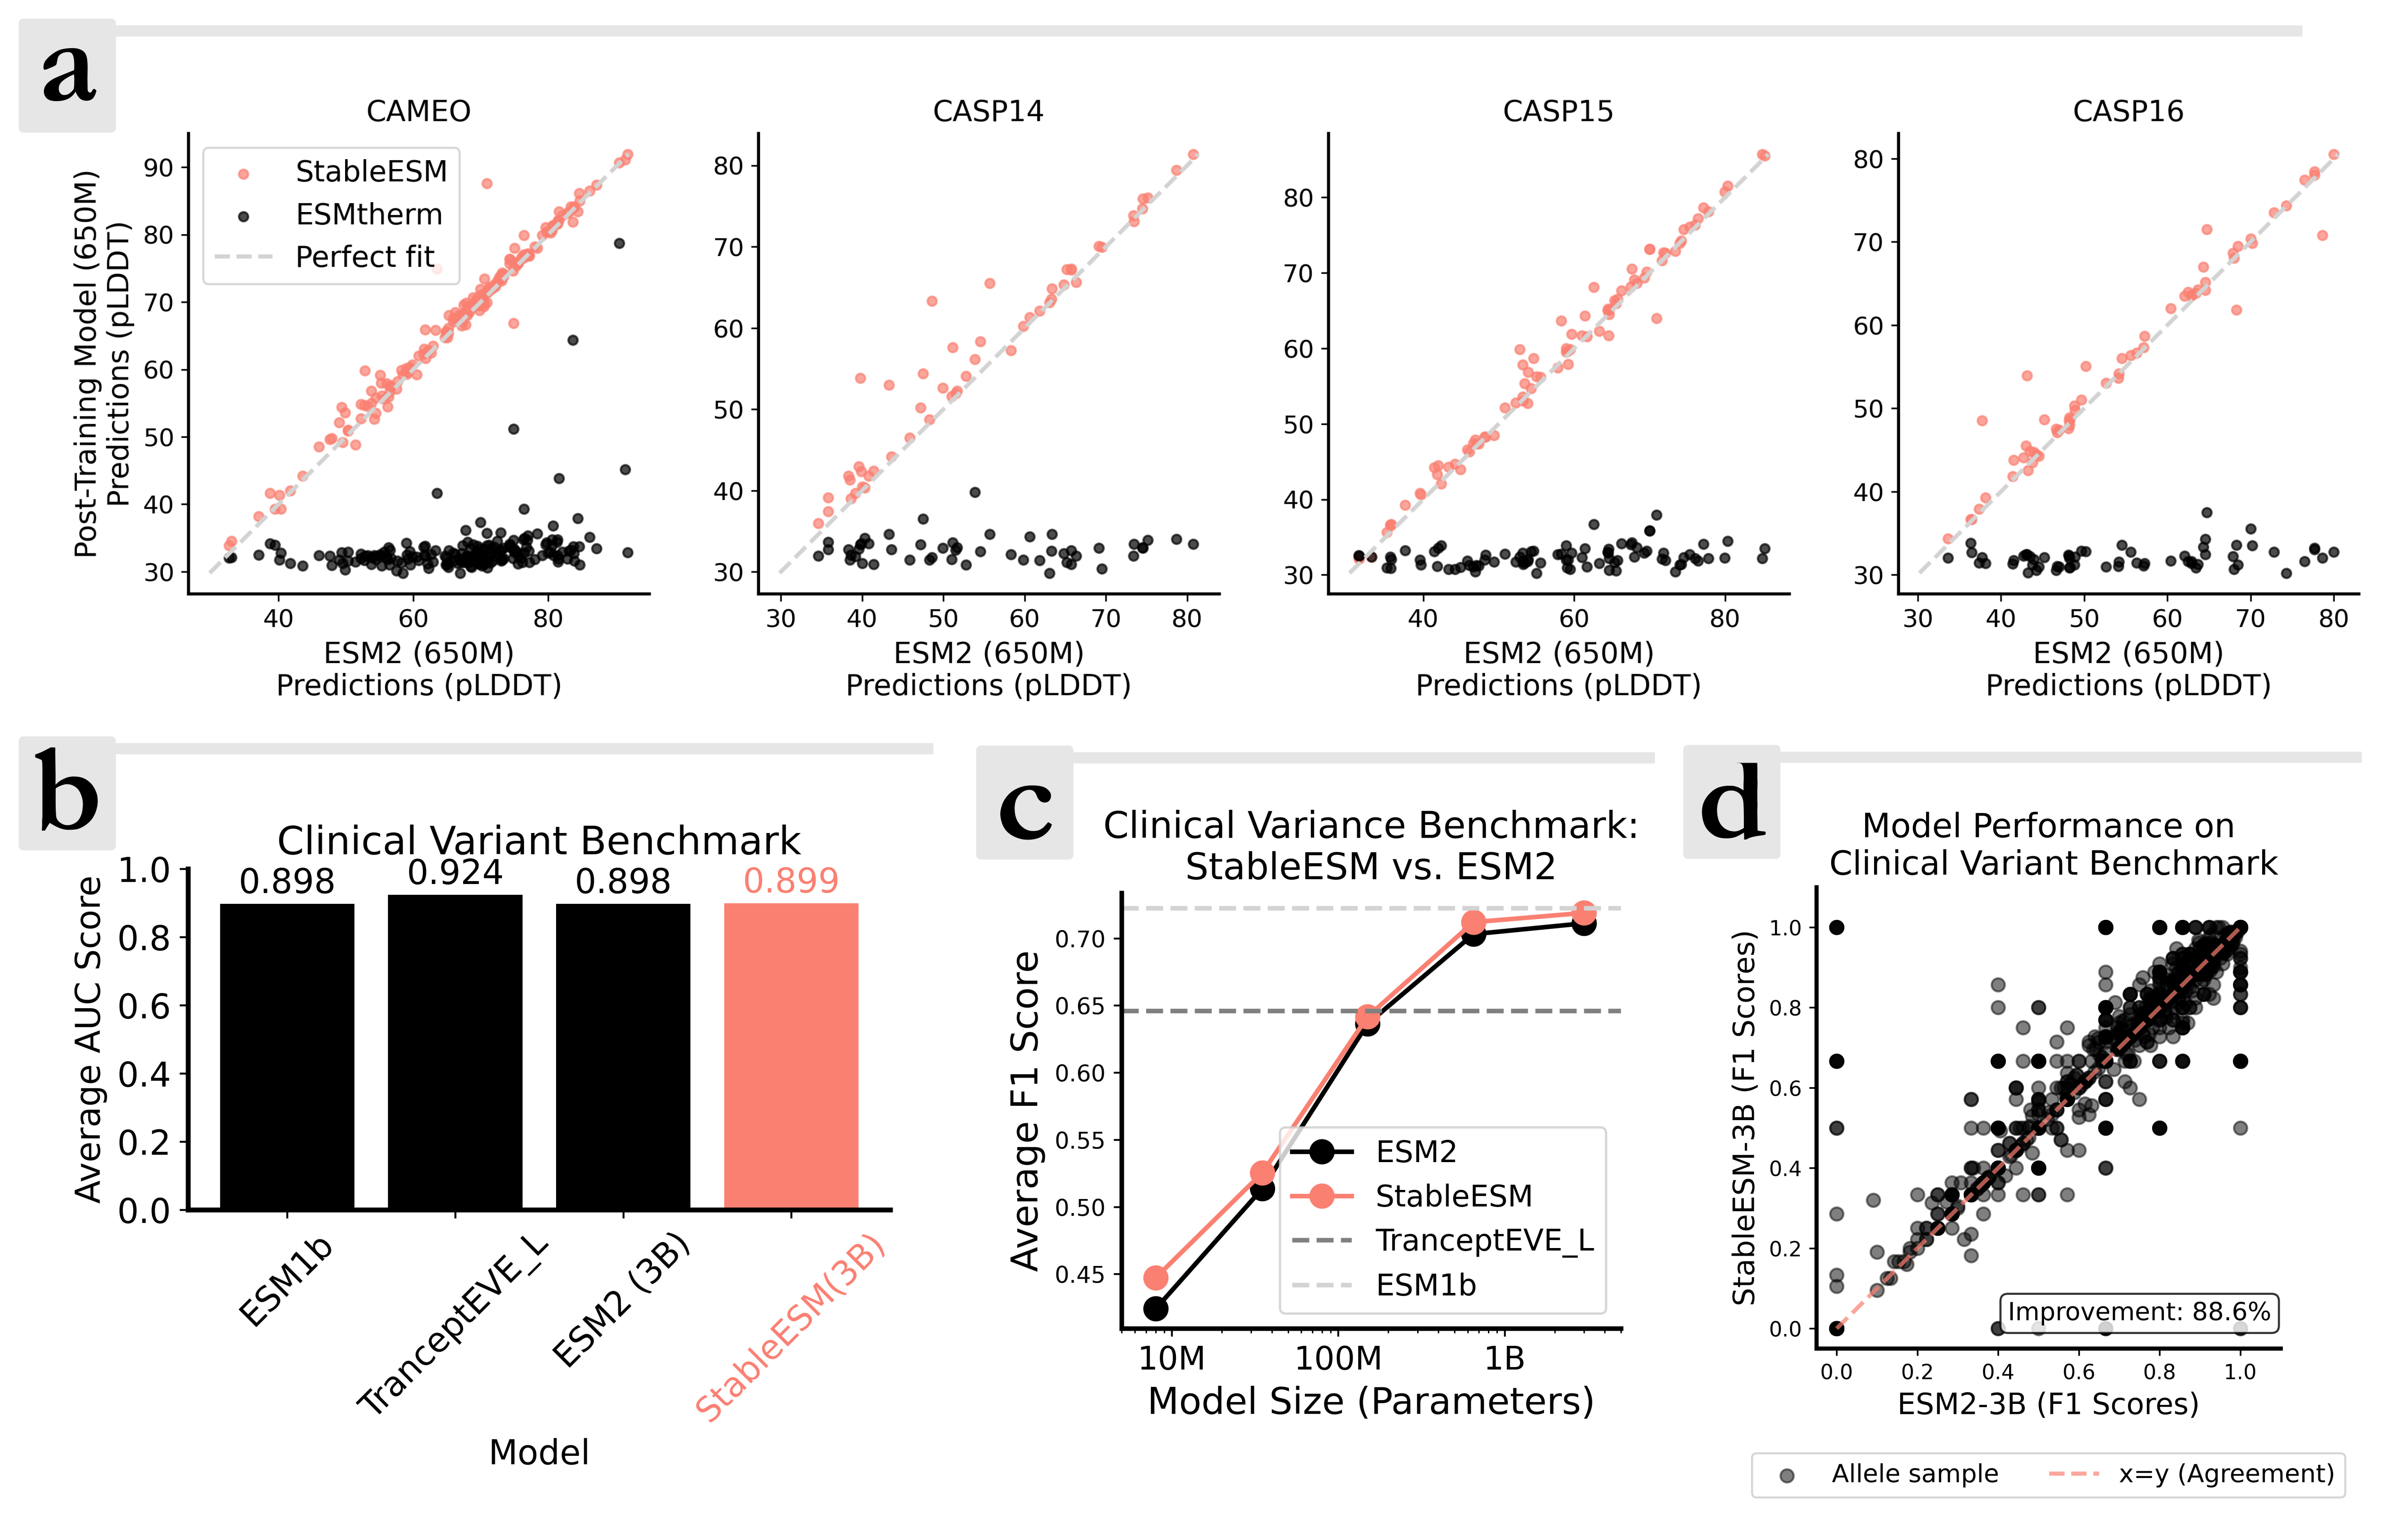
\includegraphics[width=\textwidth]{figures/Figure_3.png}
    \caption{\textbf{Direct Preference Optimization avoids catastrophic forgetting while supervised fine-tuning degrades performance.} \textbf{(a)} Structure prediction performance on CASP14-16 benchmarks shows ESM$_{Therm}$ (supervised fine-tuning) degrades performance while StableESM (DPO) maintains equivalent performance to baseline ESM2. \textbf{(b)} Clinical variant classification performance demonstrates preserved pathogenicity prediction capabilities. \textbf{(c)} Scaling analysis of clinical variant performance shows StableESM maintains strong performance across model sizes compared to ESM2. \textbf{(d)} Comprehensive comparison on clinical benchmarks confirms that preference alignment preserves critical clinical variant prediction abilities.}
    \label{fig: cata_forget}
\end{figure}




\subsection{Transfer to unrelated protein tasks: disorder region and solubility prediction}

A key question is whether stability-aligned representations transfer to protein properties beyond mutation effect prediction. To test this, we evaluated StableESM on two tasks entirely unrelated to the stability alignment objective: per-residue disorder region prediction and sequence-level solubility classification. Neither task was targeted during DPO training, making any improvements a direct indicator that preference alignment produces more generally informative protein representations.

\subsubsection{Disorder region prediction}

We benchmarked StableESM representations on the CAID (Critical Assessment of Intrinsic Disorder) benchmark using a linear probing setup: a single trainable linear layer on top of frozen backbone representations (Methods~\ref{sec:disorder_prediction}). This setup isolates the quality of learned representations by controlling for model capacity—the same linear head architecture, training data, and hyperparameters are used across all backbones.

StableESM consistently outperforms ESM2 across all model sizes (8M to 650M parameters) on mean F1 score across CAID benchmark proteins (Figure~\ref{fig:disorder_solubility}a). Both models substantially outperform the ESM$_{Therm}$ baseline (mean F1 = XXX) and the one-hot encoding control (mean F1 = XXX), confirming that the improvements stem from learned representations rather than trivial sequence features. At 650M parameters, StableESM achieves a mean F1 of XXX compared to ESM2's XXX, with XXX\% of individual CAID domains showing improved or equal F1 scores (Figure~\ref{fig:disorder_solubility}b).

The improvement on disorder prediction is particularly notable because intrinsically disordered regions are defined by their lack of stable tertiary structure—the opposite of what the stability alignment objective directly targets. This suggests that DPO alignment teaches the model more nuanced representations of sequence-structure relationships, including the ability to distinguish ordered from disordered regions, rather than simply biasing all predictions toward stability.

\subsubsection{Solubility prediction}

We similarly evaluated StableESM on binary solubility classification using a linear probe with mean pooling over frozen per-residue representations (Methods~\ref{sec:disorder_prediction}). StableESM representations yield improved solubility classification performance compared to ESM2 across model sizes, with StableESM-650M achieving an AUROC of XXX compared to ESM2-650M's XXX (Figure~\ref{fig:disorder_solubility}c). As with disorder prediction, ESM$_{Therm}$ representations show degraded performance relative to the base ESM2 model, further demonstrating that supervised fine-tuning compromises general representation quality while DPO preserves and enhances it.

The transfer to both disorder and solubility prediction reinforces a consistent pattern throughout our results: DPO-based alignment produces representations that capture fundamental principles of protein biophysics rather than narrowly optimizing for the training objective. This emergent generalization stands in contrast to ESM$_{Therm}$, where supervised fine-tuning on the same stability data leads to representations that are worse than the base model on nearly every task outside the specific training objective.

\begin{figure}[H]
    \centering
    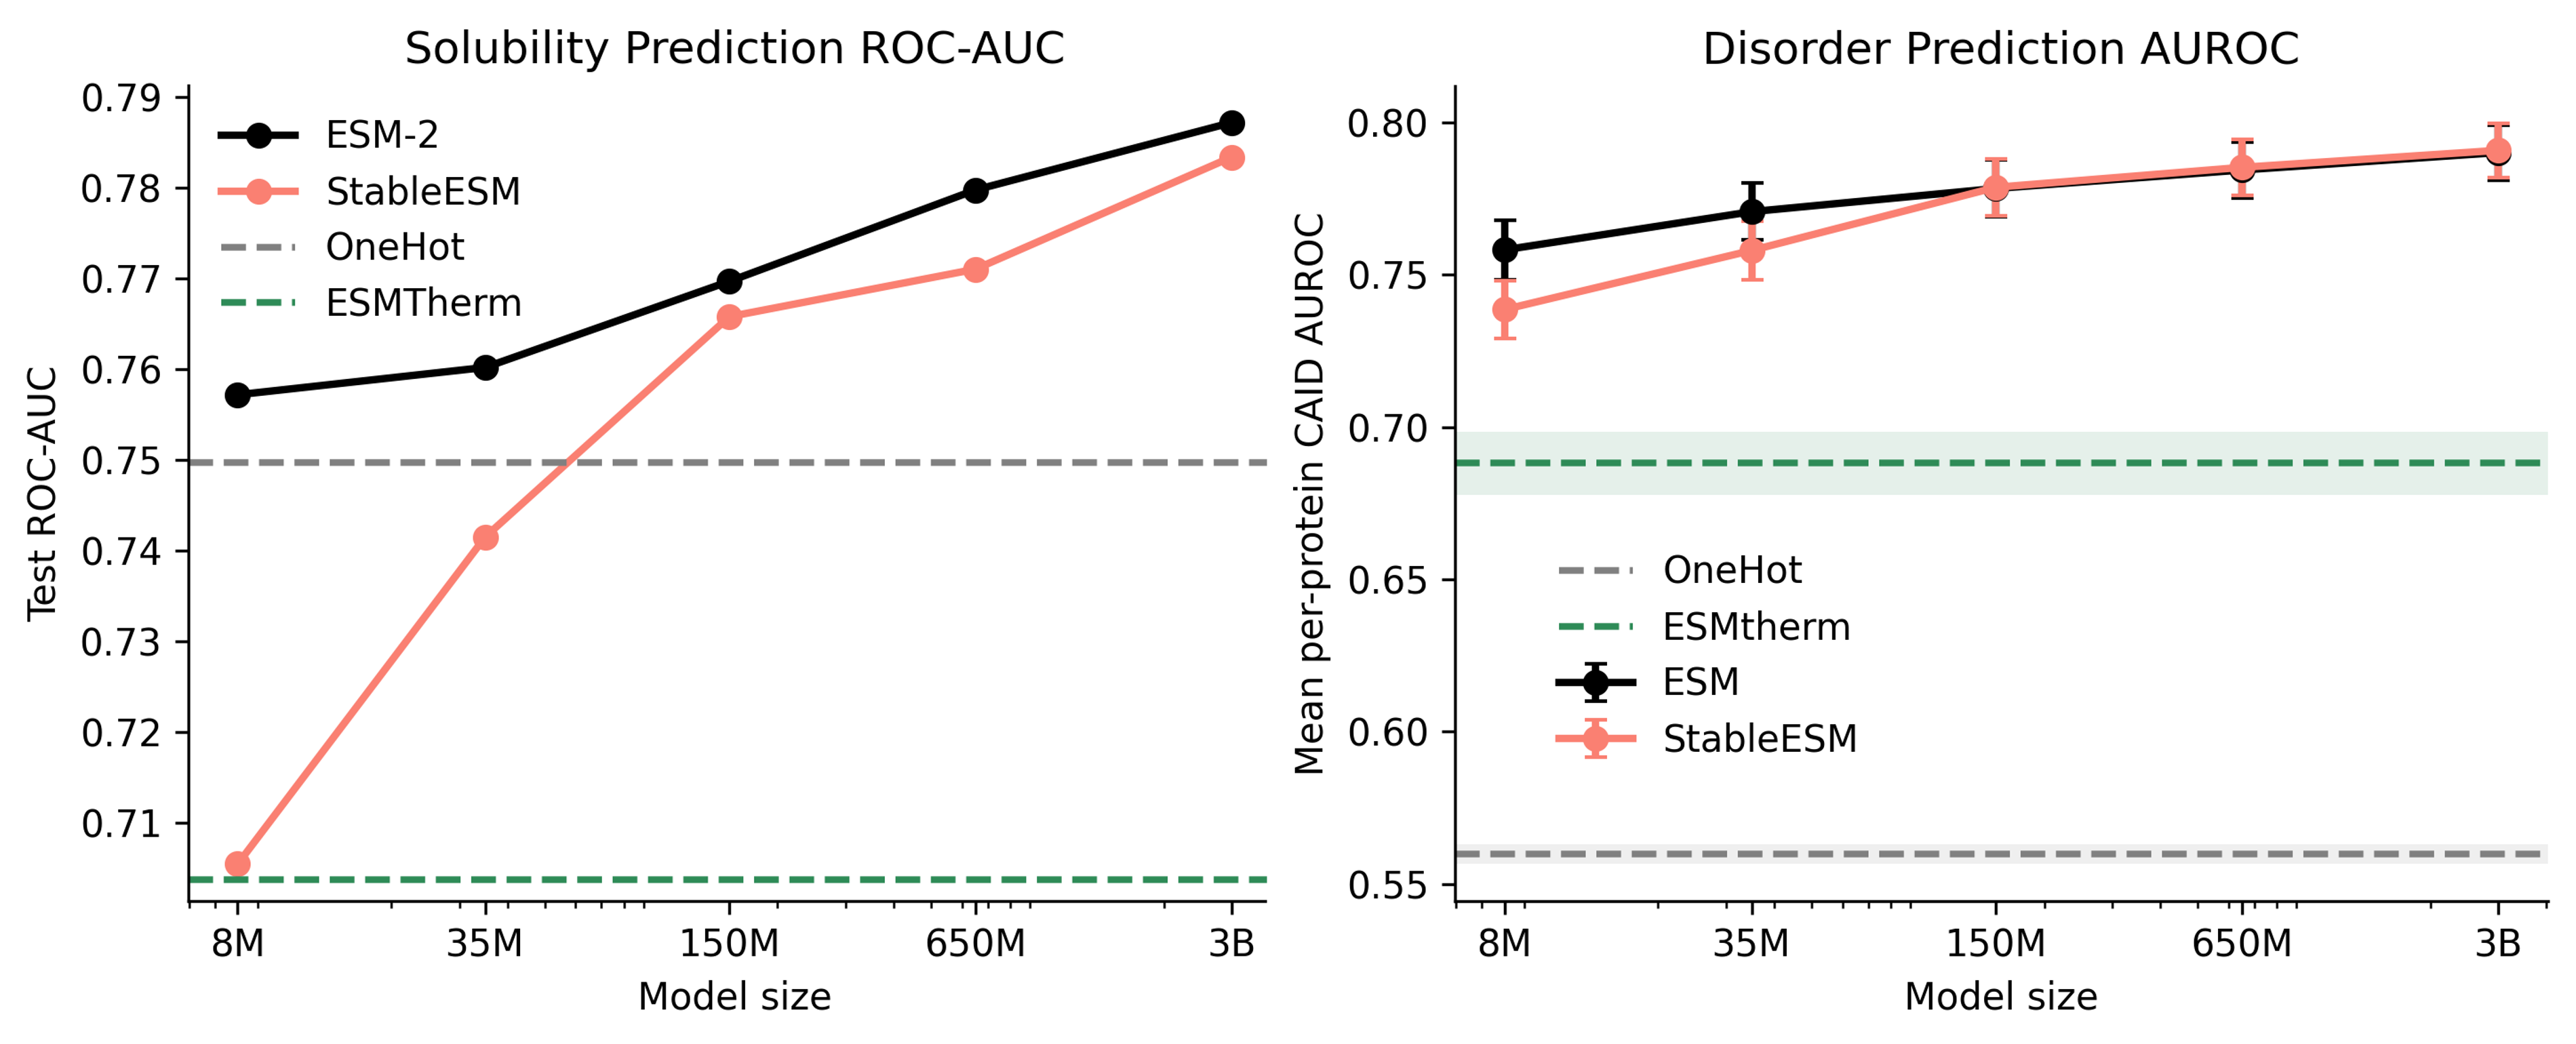
\includegraphics[width=\textwidth]{figures/Figure_X_disorder_solubility.png}
    \caption{\textbf{StableESM representations transfer to unrelated protein prediction tasks.} \textbf{(a)} Mean F1 scores for per-residue disorder region prediction on the CAID benchmark across model sizes. StableESM (red) consistently outperforms ESM2 (black) and baselines (ESM$_{Therm}$, one-hot) using identical linear probe architecture and training procedure. \textbf{(b)} Per-domain F1 score comparison between StableESM and ESM2 at 650M parameters, with points above the diagonal indicating domains where StableESM provides improved disorder prediction. \textbf{(c)} Solubility classification performance (AUROC) across model sizes, demonstrating that stability-aligned representations also improve sequence-level property prediction. All evaluations use frozen backbone representations with a single trainable linear layer to isolate representation quality.}
    \label{fig:disorder_solubility}
\end{figure}


\subsection{Designing thermostable multicopper oxidases with StableESM-guided directed evolution}

To validate StableESM's predictive accuracy beyond computational benchmarks, we experimentally tested designed mutations in laccase (CotA) from \textit{Bacillus subtilis}, a multicopper oxidase family not represented in the preference alignment dataset.
We selected mutations based on StableESM predictions using a machine learning-directed evolution framework (Algorithm~\ref{alg:ml_directed_evolution}, Methods~\ref{sec:oxidase_design}), comparing three design strategies: (1) overlap mutants where both StableESM and ESM2 predict stabilizing effects (LLR $\geq 0$ for both models), (2) StableESM-unique mutants where StableESM predicts stabilizing effects but ESM2 does not (LLR$_{\text{StableESM}} \geq 0$ and LLR$_{\text{ESM2}} < 0$), and (3) ESM2 greedy sampling as baseline.

\subsubsection{Experimental validation of single-mutation predictions}

Experimental enzyme activity assays confirmed StableESM's predictions, with designed mutants demonstrating enhanced thermostability across temperature conditions (Figure~\ref{fig:exp_validation}).
Notably, overlap mutant T261F, predicted as stabilizing by both models (LLR $> 0$), maintained superior activity relative to wild-type at 65$^\circ$C and retained approximately 2-fold higher activity than wild-type even at the extreme condition of 85$^\circ$C.
Critically, our results reveal that positive log-likelihood ratios from both StableESM and ESM2 are required to obtain thermally stable oxidases that maintain or improve catalytic activity at elevated temperatures.
This finding suggests that ESM2's log-likelihood landscape captures functional constraints related to catalytic activity, while StableESM's aligned landscape is more specifically tuned to thermodynamic stability.
Mutations predicted as stabilizing only by StableESM (LLR$_{\text{StableESM}} \geq 0$, LLR$_{\text{ESM2}} < 0$) may stabilize the protein fold but compromise catalytic function, consistent with the interpretation that these mutations fall in regions where stability gains come at the cost of disrupting functionally important interactions.
The overlap between both models' positive predictions thus identifies a sweet spot in sequence space where mutations are both thermodynamically stabilizing and functionally permissive.

These results validate that StableESM learns transferable stability principles that generalize to completely unseen protein families, and that combining StableESM with the base ESM2 model enables accurate prediction of functional improvements in distantly related proteins.
A second round of single-mutation experiments is currently underway to further explore the overlap design strategy and identify additional thermostable variants with maintained or improved activity.

\subsubsection{In silico design validation through machine learning-directed evolution}

Additionally, we demonstrate StableESM's utility in large-scale protein design through machine learning-directed evolution on multicopper oxidase (PDB: 1GSK), a 513 amino acid protein not represented in any form within the preference alignment dataset (Methods~\ref{sec:oxidase_design}).
Using TempBERTura~\citep{rodella2024temberture} for thermal stability evaluation, StableESM greedy design achieved the highest predicted $T_m$ of 74.2$^\circ$C with high confidence (0.978), representing a 15.4$^\circ$C improvement over the wild-type predicted $T_m$ of 58.8$^\circ$C.
The StableESM unique sampling strategy achieved a predicted $T_m$ of 61.9$^\circ$C with even higher confidence (0.981), demonstrating that StableESM identifies stabilizing mutations missed by the base model.
ESM2 greedy design reached a similar predicted $T_m$ of 73.7$^\circ$C but with substantially lower confidence (0.686), highlighting the value of preference alignment for confident predictions.

Critically, StableESM and ESM2 greedy designs differed significantly from each other (86.2\% similarity, 71 mismatches) despite making similar numbers of edits ($N = 400$), demonstrating that preference alignment fundamentally alters sequence space exploration even for completely unseen proteins distant from the training data.
Structural quality assessment using ColabFold confirmed that all stabilizing designs maintained high predicted structural integrity with mean pLDDT scores above 91 (Figure~\ref{fig:insilico_validation}).

\begin{figure}[H]
    \centering
    \includegraphics[width=\textwidth]{figures/Figure_4.png}
    \caption{\textbf{Experimental validation of StableESM mutant predictions.} \textbf{(a)} Machine learning-directed evolution framework using StableESM predictions to guide exploration of fitness landscapes. \textbf{(b)} Enzyme activity measurements for multicopper oxidase variants at elevated temperatures. Overlap mutant T261F, computationally predicted as stabilizing by both models, demonstrates enhanced thermostability with maintained activity at 65$^\circ$C and 2-fold improvement over wild-type at 85$^\circ$C, validating the accuracy of stability predictions.}
    \label{fig:exp_validation}
\end{figure}

%\begin{figure}[H]
%    \centering
%    \includegraphics[width=\textwidth]{figures/Figure_5.png}
%    \caption{\textbf{In silico validation of StableESM through thermostable protein design.} \textbf{(a)} In silico results comparing greedy vs. preference-aligned design strategies, showing StableESM identifies beneficial mutations achieving higher predicted melting temperatures and stability using TempBERTura. \textbf{(b)} Designed protein structures computationally predicted to possess improved thermostability across multiple variants, validating practical utility for experimental protein engineering.}
%    \label{fig:insilico_validation}
%\end{figure}


\section{Discussion}
\label{sec:discussion}

StableESM establishes that preference optimization with experimental stability data can fundamentally improve how protein language models predict mutation effects, generalize to unseen proteins, and explore fitness landscapes for protein design.
The approach addresses multiple limitations of current protein language models simultaneously: performance improvements are consistent across all model sizes from 8M to 3B parameters, generalization extends to completely novel protein families and sequence lengths far beyond the training distribution, and critically, the alignment procedure avoids catastrophic forgetting across structure prediction, clinical variant assessment, and functional prediction benchmarks.

A central finding is that preference alignment restores scaling laws for mutation effect prediction in protein language models.
While vanilla ESM2 performance saturates or deteriorates from 650M to 3B parameters on out-of-distribution benchmarks—consistent with reports that larger models overfit to phylogenetic noise rather than functional constraints~\citep{weinstein2022non,hou2025understanding}—StableESM shows continued improvement with scale.
This suggests that larger protein language models possess latent capabilities for understanding protein stability and function that are not accessed through masked language modeling alone but can be unlocked through targeted post-training alignment.
The $\sim$1 million preference pairs used here represent a tiny fraction of the data used during pretraining, yet they fundamentally alter model behavior, paralleling the observation in natural language processing that relatively small alignment datasets can redirect large pretrained models toward substantially improved task performance~\citep{ouyang2022training}.

The contrast between DPO-based alignment and supervised fine-tuning reveals why the choice of post-training objective matters.
ESM$_{Therm}$, trained with a regression head on the same stability data, achieves competitive performance on its specific training task but catastrophically degrades on structure prediction, clinical variant assessment, and all ProteinGym functional categories when evaluated through log-likelihood ratios.
This pattern aligns with recent findings in natural language processing that supervised fine-tuning tends to memorize training data patterns while reinforcement learning approaches learn generalizable principles~\citep{chu2025sft}.
DPO's inherent regularization—constraining the aligned model to remain close to the reference model through the KL divergence penalty in the objective—appears essential for preserving the rich evolutionary representations learned during pretraining while selectively enhancing the model's sensitivity to stability-relevant features.

The emergent transfer of stability alignment to unrelated tasks provides evidence that DPO produces more generally informative protein representations rather than narrowly optimizing for stability prediction.
StableESM improves performance on disorder region prediction, solubility classification, expression prediction, and binding prediction—none of which were targeted during training.
This transfer is particularly striking for disorder prediction, where intrinsically disordered regions are defined by their lack of stable structure.
The improvement suggests that preference alignment teaches the model to better distinguish between ordered and disordered sequence contexts as part of learning a more refined understanding of sequence-structure-stability relationships.

Our experimental validation in multicopper oxidase engineering reveals a practical framework for using aligned and unaligned models in combination for protein design.
The key finding that positive log-likelihood ratios from both StableESM and ESM2 are required to identify mutations that are both thermally stabilizing and catalytically active has direct implications for how these models should be deployed.
ESM2's log-likelihood landscape appears to capture functional constraints related to catalytic activity—reflecting the evolutionary pressures encoded during pretraining—while StableESM's aligned landscape is more specifically tuned to thermodynamic stability.
Mutations where only StableESM predicts stabilizing effects (LLR$_{\text{StableESM}} \geq 0$, LLR$_{\text{ESM2}} < 0$) may stabilize the protein fold but disrupt functionally important interactions, while the overlap region identifies mutations that satisfy both stability and functional constraints simultaneously.
This complementary relationship between aligned and base models suggests that post-training alignment does not simply replace the base model's knowledge but adds a distinct and complementary perspective on sequence-function relationships.

The 86.2\% sequence similarity between StableESM and ESM2 greedy designs—despite comparable numbers of edits—demonstrates that preference alignment fundamentally alters how models navigate sequence space.
This landscape alteration has practical implications: aligned models identify beneficial mutations and design strategies that would be entirely missed by unaligned approaches.
The experimental confirmation that designed variants maintain or exceed wild-type activity across normal (25$^\circ$C), thermophilic (65$^\circ$C), and extremophilic (85$^\circ$C) temperature conditions validates that these computational predictions translate to measurable functional improvements in proteins completely absent from the training data.

Several limitations of our current approach warrant discussion.
First, our preference dataset is constructed exclusively from stability measurements ($\Delta\Delta G$ and $\Delta T_m$), which may introduce biases toward stability-related features at the expense of other functional properties.
The observed improvements on non-stability tasks suggest this concern is partially mitigated by DPO's regularization, but multi-objective alignment incorporating diverse functional measurements could produce even more broadly capable models.
Second, while we demonstrate generalization to unseen protein families and lengths substantially beyond training, the degree of generalization likely depends on the diversity and coverage of the preference dataset—expanding to more diverse protein architectures and fold types may further extend generalization capabilities.
Third, our experimental validation is currently limited to single-mutation effects in a single protein system; broader experimental campaigns across multiple protein families and combinatorial mutations would strengthen the evidence for practical utility.

Future work should explore several directions.
Extending preference alignment to incorporate experimental measurements of activity, binding affinity, solubility, and expression level could enable multi-objective protein optimization.
The overlap mutant strategy—requiring agreement between aligned and base models—could be generalized to combinations of models aligned to different properties, providing a principled approach to multi-property protein design.
Investigating preference learning objectives that explicitly capture epistatic interactions through higher-order mutational data could improve predictions for combinatorial protein engineering.
As experimental datasets continue to grow through initiatives like deep mutational scanning atlases~\citep{fowler2023atlas}, preference-based alignment may become a standard component of protein foundation model development, enabling models that not only understand evolutionary patterns but can effectively navigate fitness landscapes for practical protein design.

\section{Code and Data Availability}
\label{sec:code_data}

All code for training StableESM, running inference, evaluating on benchmarks, and reproducing downstream task experiments (disorder prediction, solubility prediction, forward evolution) is available at \url{https://github.com/PraljakReps/StableESM} under the MIT license.
The repository includes configuration files, SLURM scripts for multi-GPU training, and all 39 analysis notebooks used to generate the figures and results in this paper.

Pre-trained StableESM checkpoints (8M, 35M, 150M, 650M, and 3B parameters) and trained downstream linear probe checkpoints for disorder and solubility prediction are available for download via Google Drive (see \texttt{checkpoints/README.md} in the code repository).
The curated preference dataset containing $\sim$1 million mutations across 1,154 protein domains, along with all evaluation datasets (ProteinGym, CAID disorder benchmark, solubility classification, and out-of-distribution FireProt data), can be downloaded using the automated script provided in the repository (\texttt{python download\_data.py --all}) or manually from Google Drive (see \texttt{data/README.md}).

The raw experimental databases used to construct the preference dataset are publicly available: MegaScale~\citep{tsuboyama2023mega}, Human Domainome 1~\citep{beltran2025site}, and FireProtDB~\citep{stourac2021fireprotdb}.
Data curation notebooks documenting the full preprocessing pipeline are included in \texttt{notebooks/data\_curation/}.

\section{Acknowledgments}
\label{sec:acknowledgements}

\section{Author Contributions}
\label{sec:author_contributions}

\section{Competing Interests}
\label{sec:competing_interests}

The authors declare no competing interests.

\bibliographystyle{plainnat}
\bibliography{biblio}

\clearpage
\newpage
\beginappendix

\tableofcontents

\starttocentries

\clearpage
\newpage

\section{Additional Figures \& Tables}
\label{sec:additional_figures_tables}


\begin{figure}[h!]
    \centering
    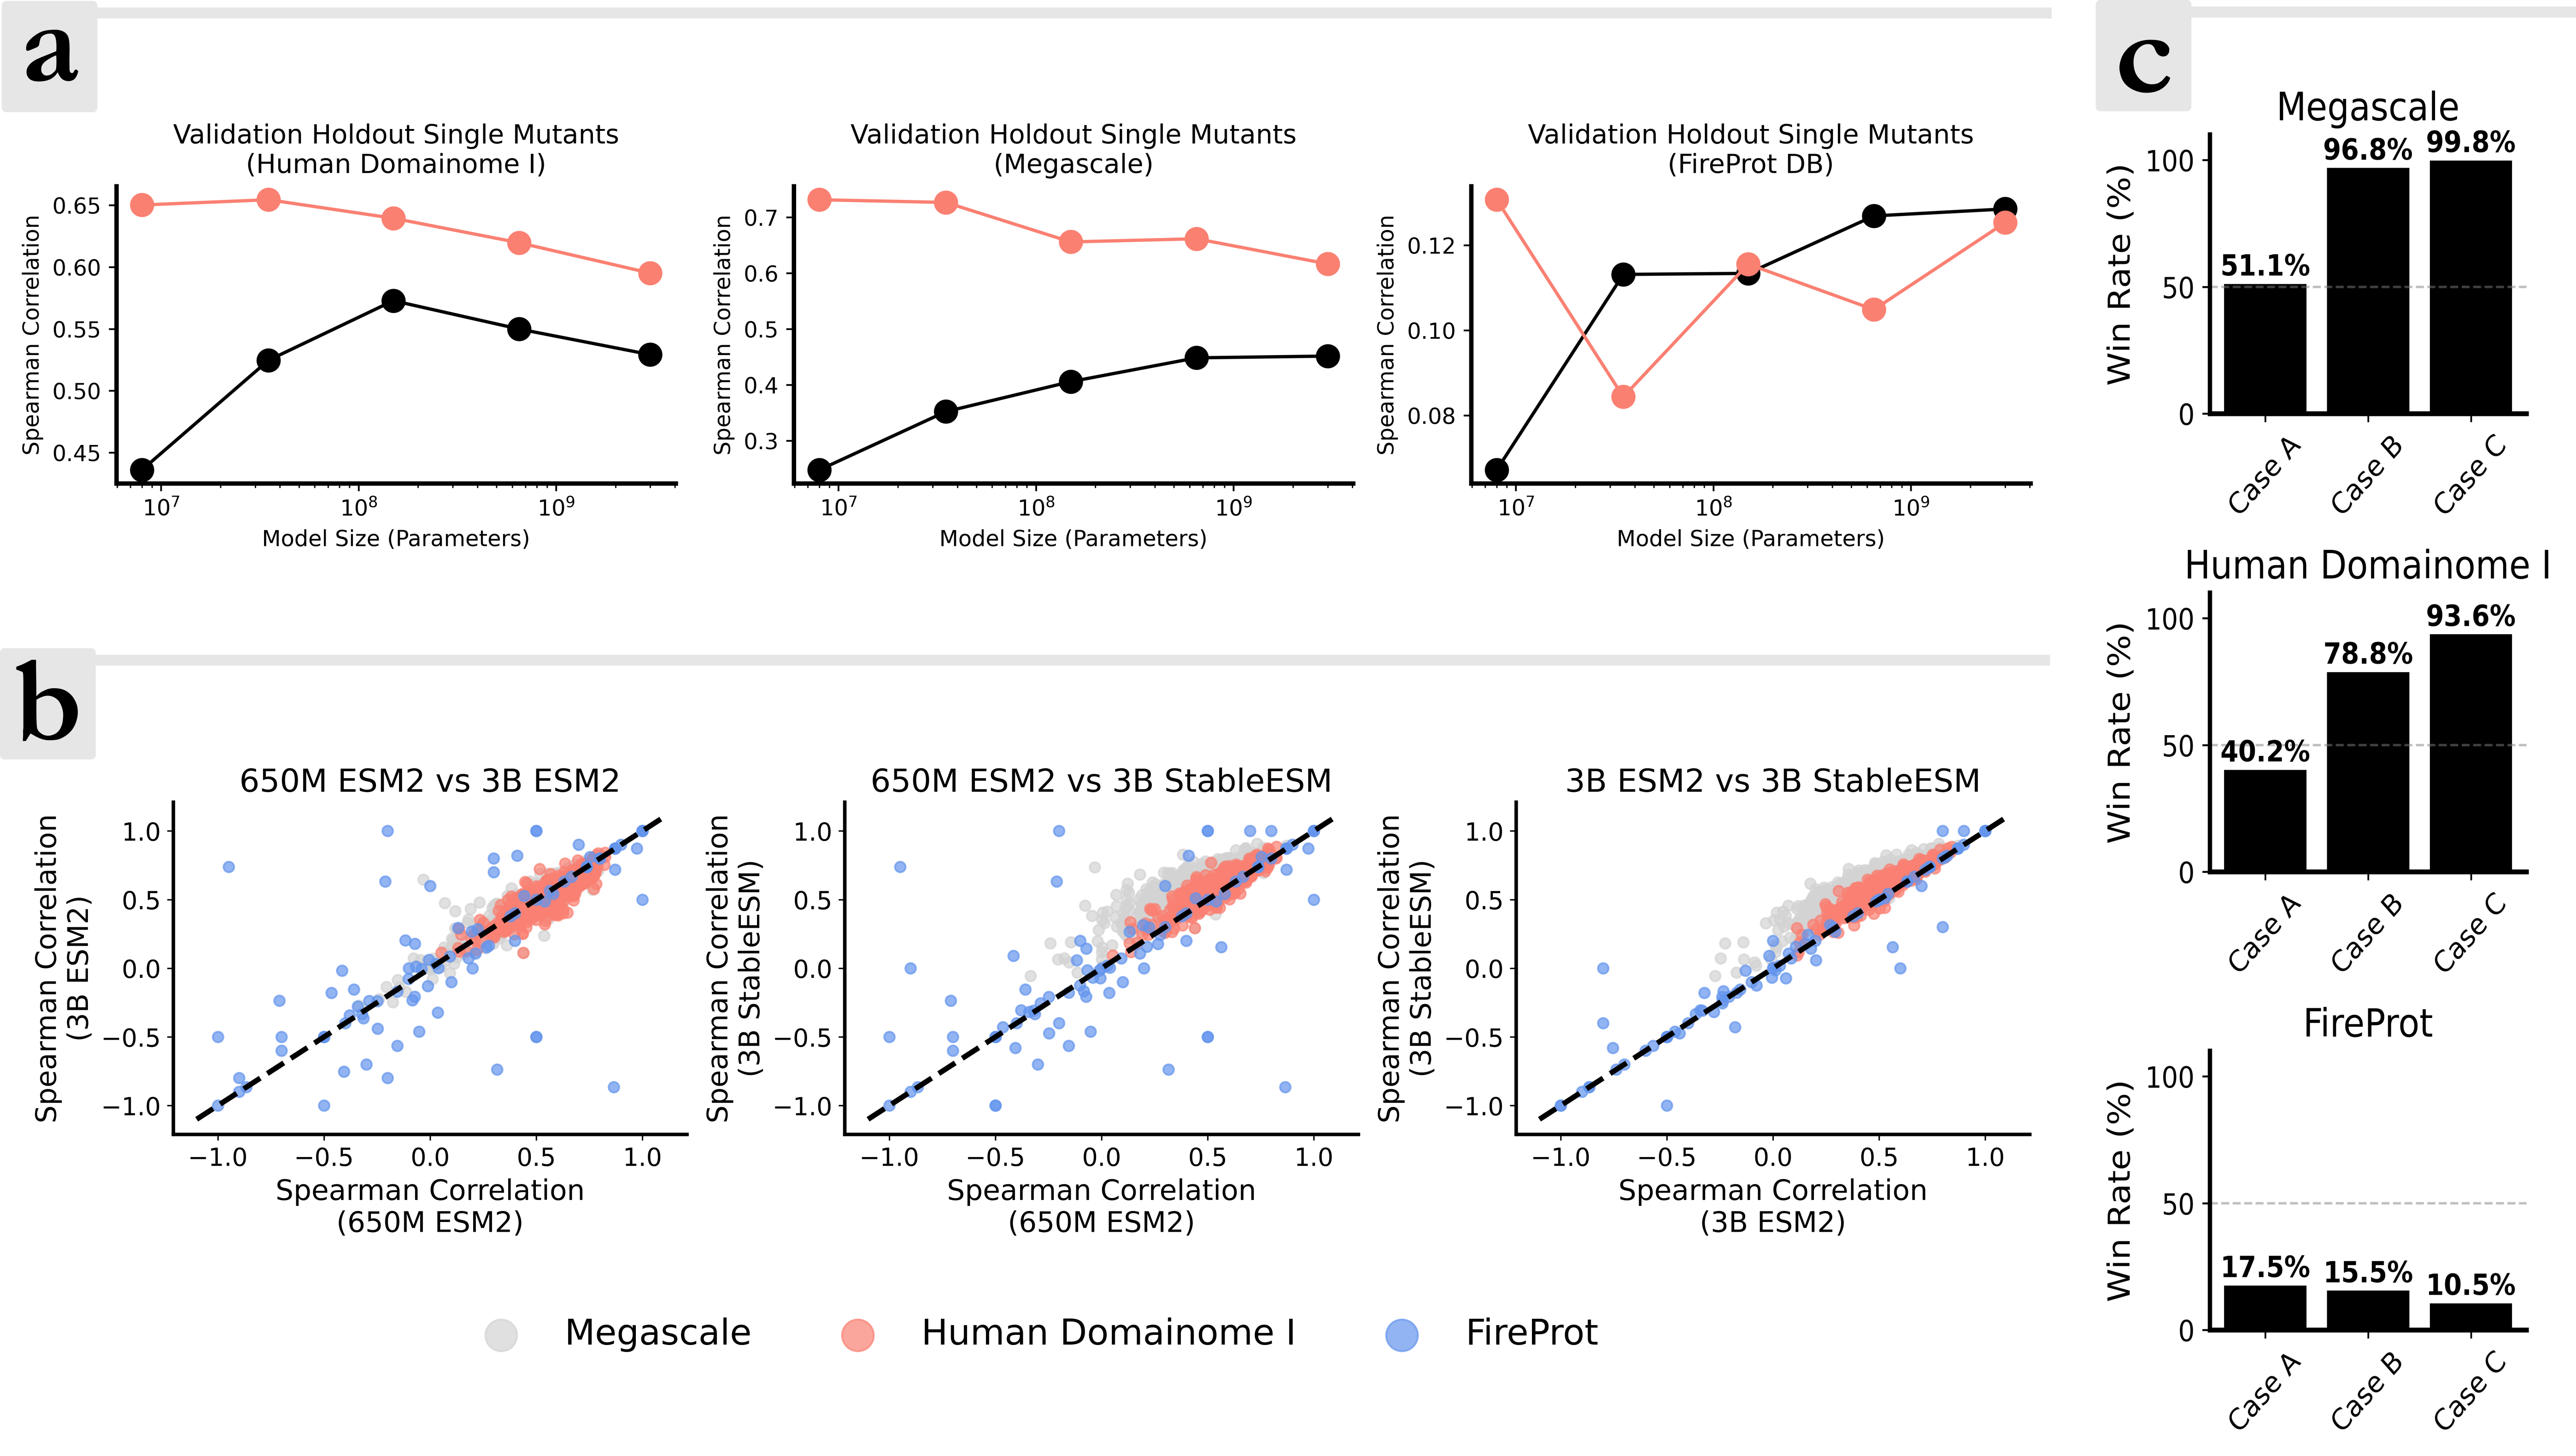
\includegraphics[width=1.0\linewidth]{figures/extended_figures/Figure_Extended_2.png}
    \caption{\textbf{StableESM demonstrates consistent validation performance improvements across datasets and model scales.} \textbf{(a)} Per-domain Spearman correlations on validation single mutants held out during training. StableESM (red) consistently outperforms ESM2 (black) across all model sizes on MegaScale and Human Domainome I datasets, with StableESM 3B achieving superior performance compared to ESM2 650M, consistent with literature reports that ESM2 3B saturates in performance against ESM2 650M while StableESM breaks this scaling limitation. FireProt shows minimal improvement, likely due to limited mutation quantity in this dataset. \textbf{(b)} Pairwise model comparisons on per-domain correlations. While scaling from ESM2 650M to 3B shows no improvement (Case A), StableESM 3B demonstrates clear superiority over both ESM2 650M (Case B) and ESM2 3B (Case C) on MegaScale and Human Domainome I datasets, with most domains falling above the diagonal. \textbf{(c)} Win-rate analysis quantifying the fraction of domains where one model outperforms another. ESM2 3B performs comparably or worse than ESM2 650M across datasets (Case A), while StableESM 3B achieves dramatic win-rates of 96.8\% and 78.8\% against ESM2 650M (Case B) and 99.8\% and 93.6\% against ESM2 3B (Case C) on MegaScale and Human Domainome I, respectively, demonstrating that preference alignment unlocks the scaling potential of larger protein language models.}
    \label{fig: eval_on_valid_holdout}
\end{figure}  

\begin{figure}[h!]
    \centering
    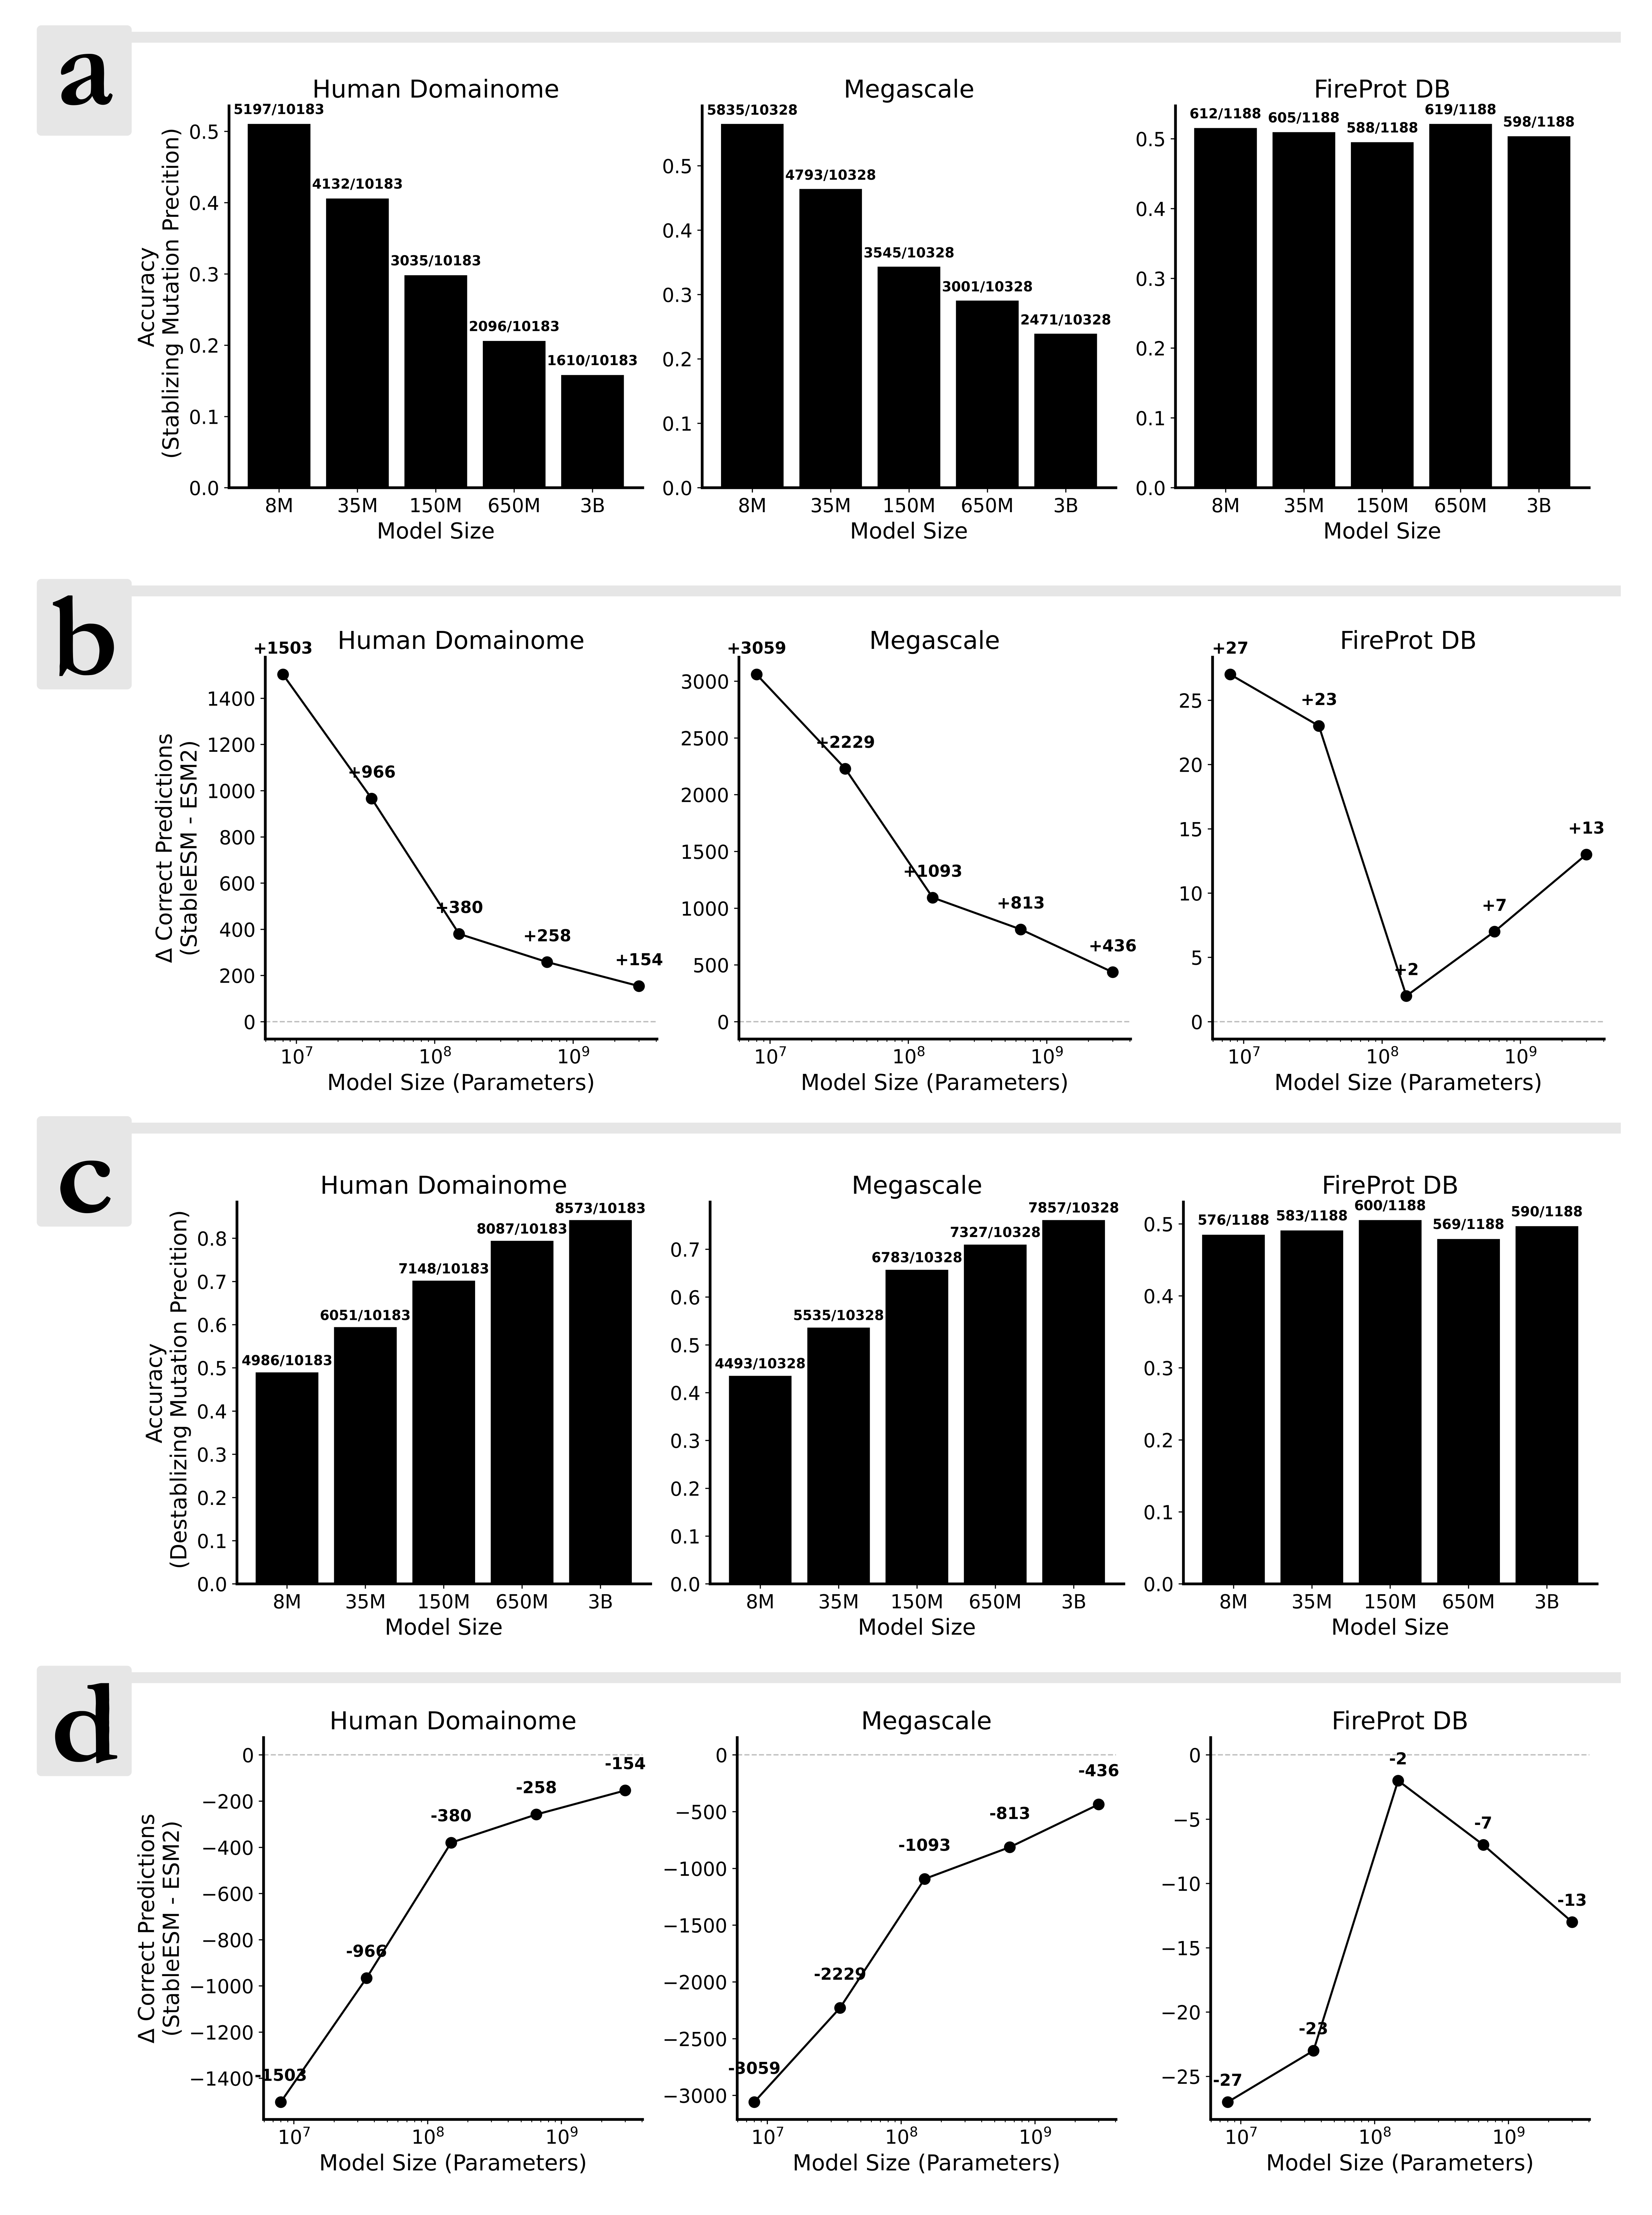
\includegraphics[width=1.0\linewidth]{figures/extended_figures/Figure_Extended_3.png}
    %\caption{}
    %\label{fig: eval_classification_on_valid_holdout}
\end{figure}



\captionof{figure}{\textbf{StableESM improves classification of both stabilizing and destabilizing mutations across model scales on validation holdout mutants, addressing known limitations in gain-of-function prediction.} \textbf{(a)} Accuracy for predicting stabilizing mutations (gain-of-function) on validation holdout mutants not seen during training. StableESM demonstrates improved performance across all model sizes on Human Domainome and Megascale datasets, with larger models achieving higher accuracy. FireProt DB shows consistently high performance across scales due to dataset characteristics. Numbers above bars indicate correct predictions over total stabilizing mutations. \textbf{(b)} Improvement in correct stabilizing mutation predictions (StableESM - ESM2) on validation holdout sets. All StableESM models show substantial gains over ESM2 baselines, with larger models being able to achieve improvements (+154, +436, +13 additional correct predictions for Human Domainome, Megascale, and FireProt DB respectively at 3B scale). \textbf{(c)} Accuracy for predicting destabilizing mutations on validation holdout mutants, where larger protein language models traditionally excel. StableESM maintains strong performance across scales while showing the expected scaling behavior where larger models achieve higher accuracy ($\sim$2x improvement from 8M to 3B), consistent with literature. \textbf{(d)} Improvement in correct destabilizing mutation predictions (StableESM - ESM2) on validation holdout sets. While larger StableESM models show modest improvements over ESM2 for deleterious predictions, smaller models like 8M exhibit high false positive predictions. These results demonstrate that larger StableESM models effectively address the known limitation of protein language models in gain-of-function prediction while preserving their established strength in identifying deleterious mutations~\citep{ertelt2025self}, suggesting that preference alignment at scale unlocks balanced performance across both stabilizing and destabilizing mutation classes.}
\label{fig: eval_classification_on_valid_holdout}


\begin{figure}[h!]
    \centering
    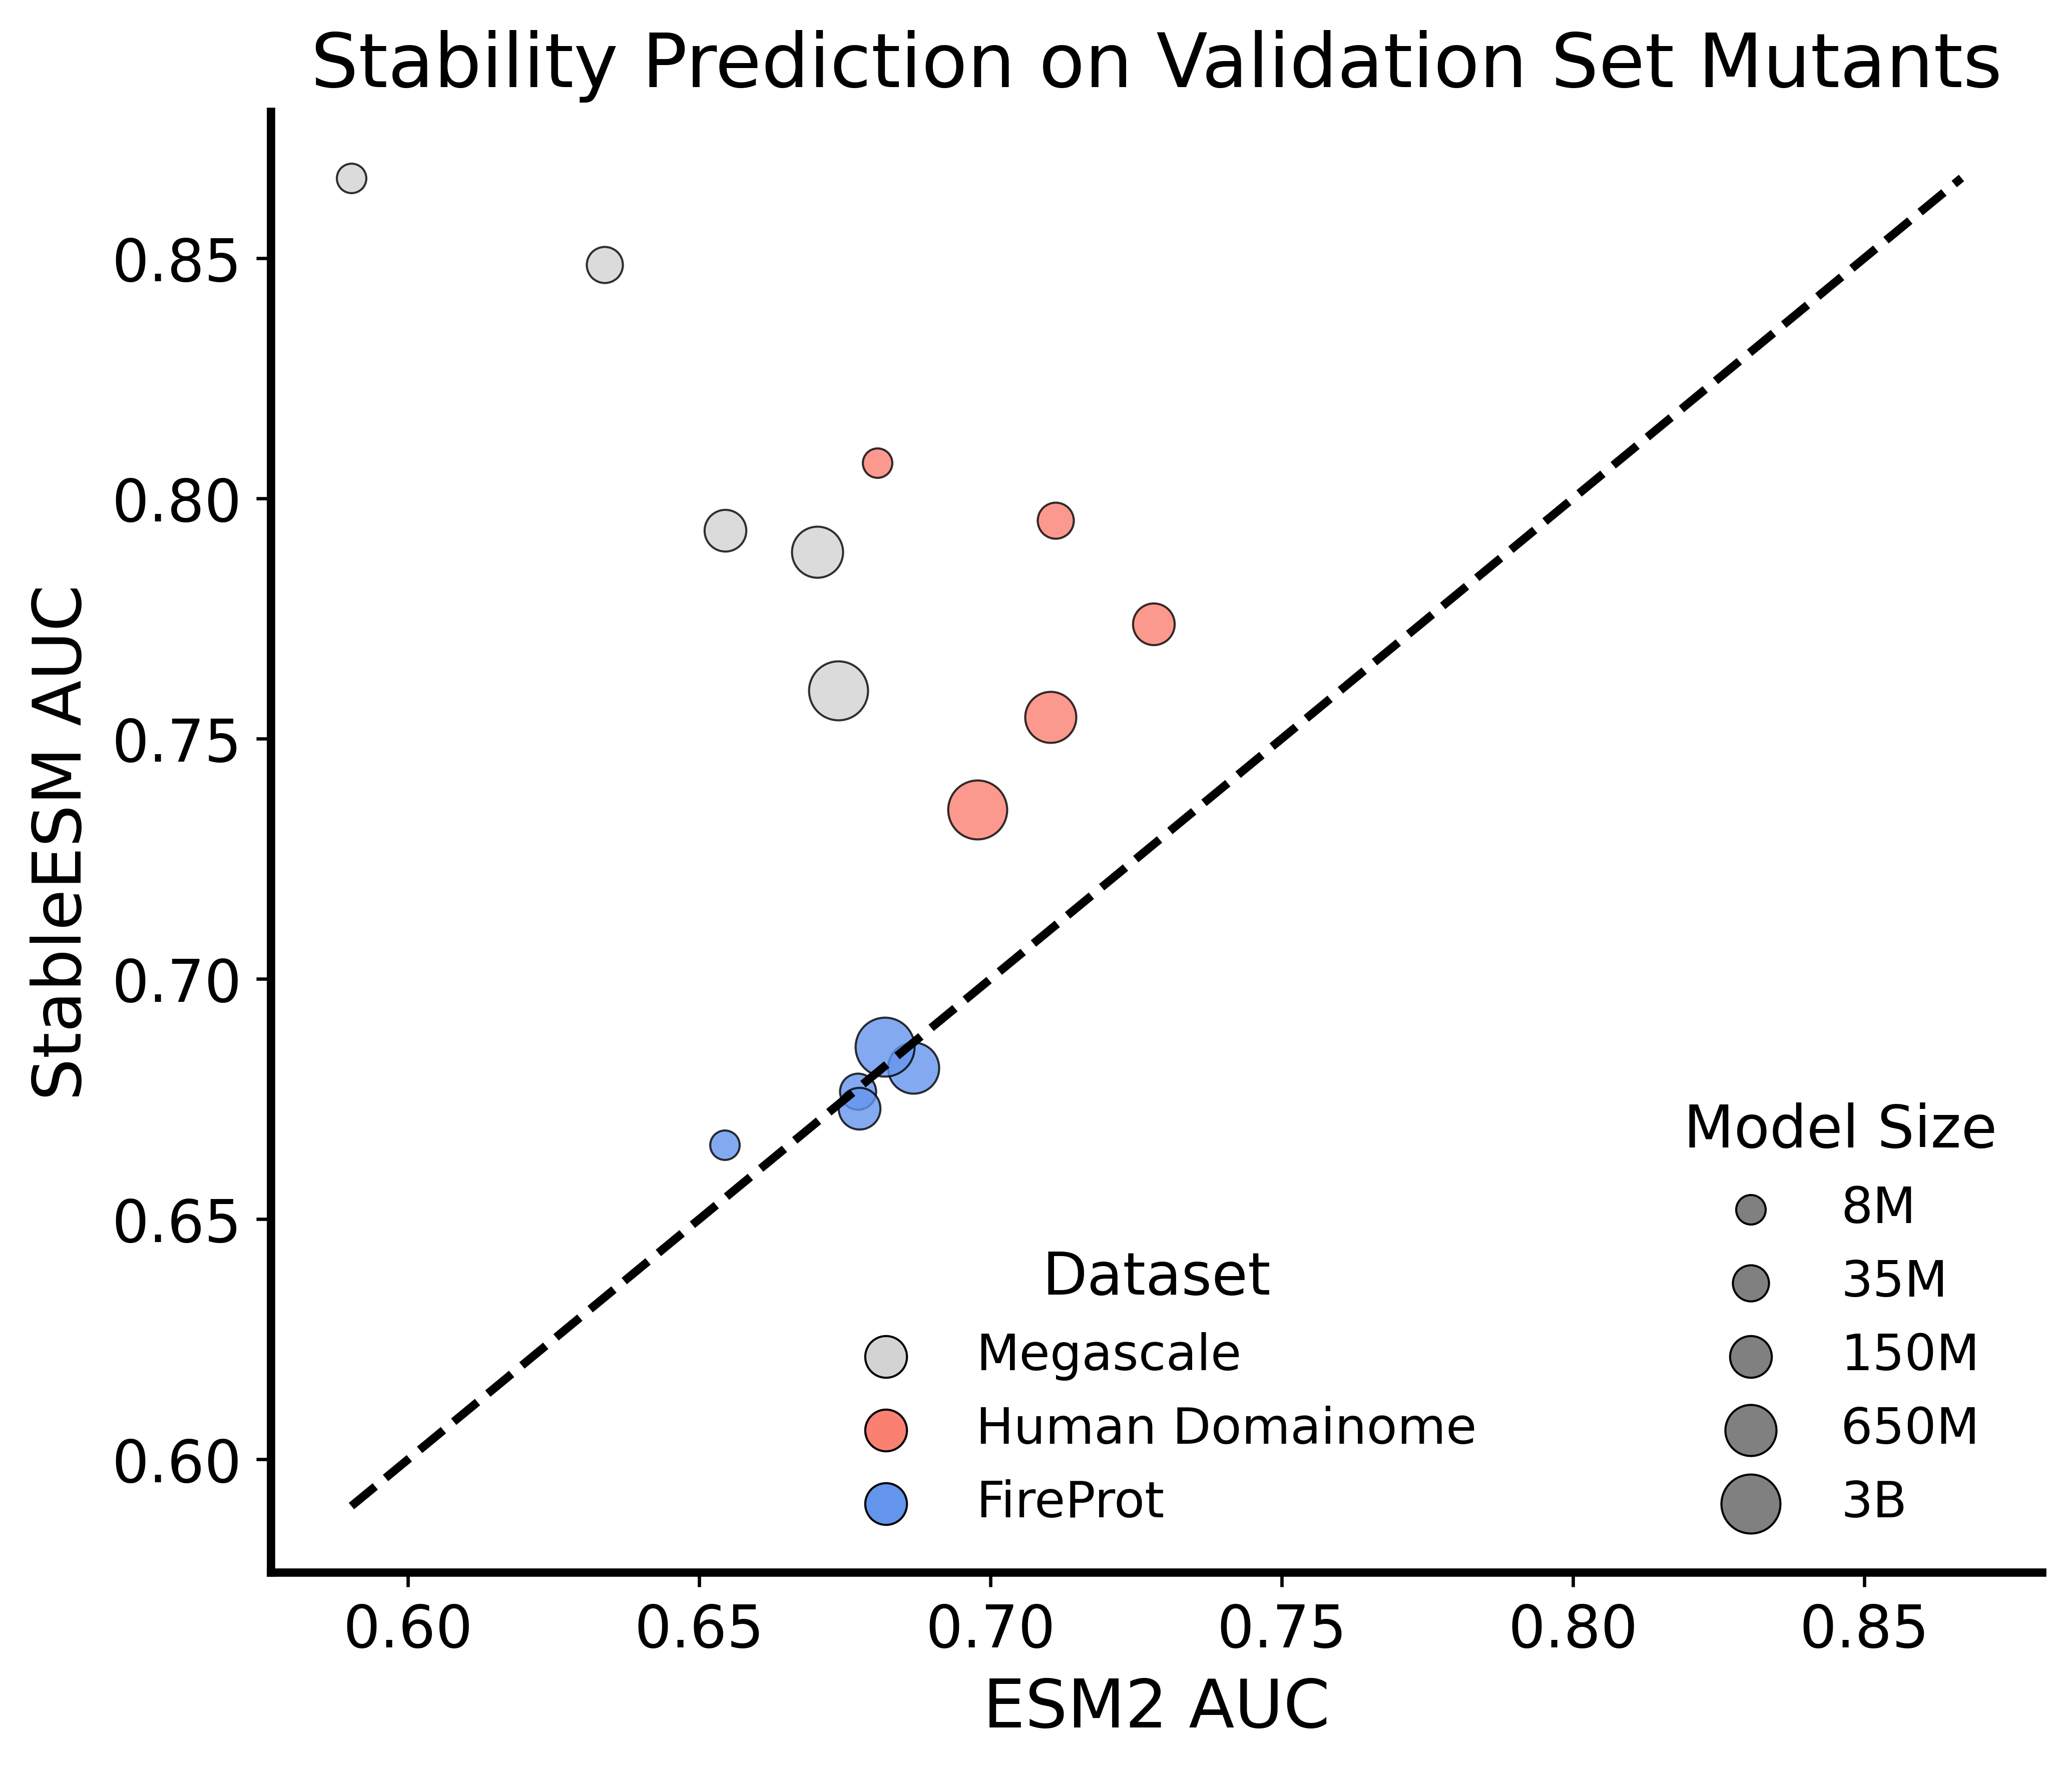
\includegraphics[width=0.6\linewidth]{figures/extended_figures/Figure_Extended4.png}
    \caption{\textbf{StableESM consistently outperforms ESM2 across all model sizes and datasets for stability prediction on validation holdout single mutants.} Each point represents AUC scores for classification of stabilizing versus destabilizing mutations, with ESM2 performance on the x-axis and StableESM performance on the y-axis. Point colors indicate dataset (grey: Megascale, red: Human Domainome, blue: FireProt) and sizes represent model scale (8M to 3B parameters). All points fall above the diagonal line, demonstrating that StableESM achieves superior classification performance compared to ESM2 across all tested conditions. Human Domainome and Megascale datasets show substantial improvements, while FireProt exhibits more modest but consistent gains. The results demonstrate that preference alignment provides robust benefits for mutation effect classification regardless of model size or dataset characteristics, with improvements ranging from  $\sim$0.01 to $\sim$0.08 AUC units across the tested conditions.}
    \label{fig: auc_comparison_val_holdout}
\end{figure}



\begin{figure}[h!]
    \centering
    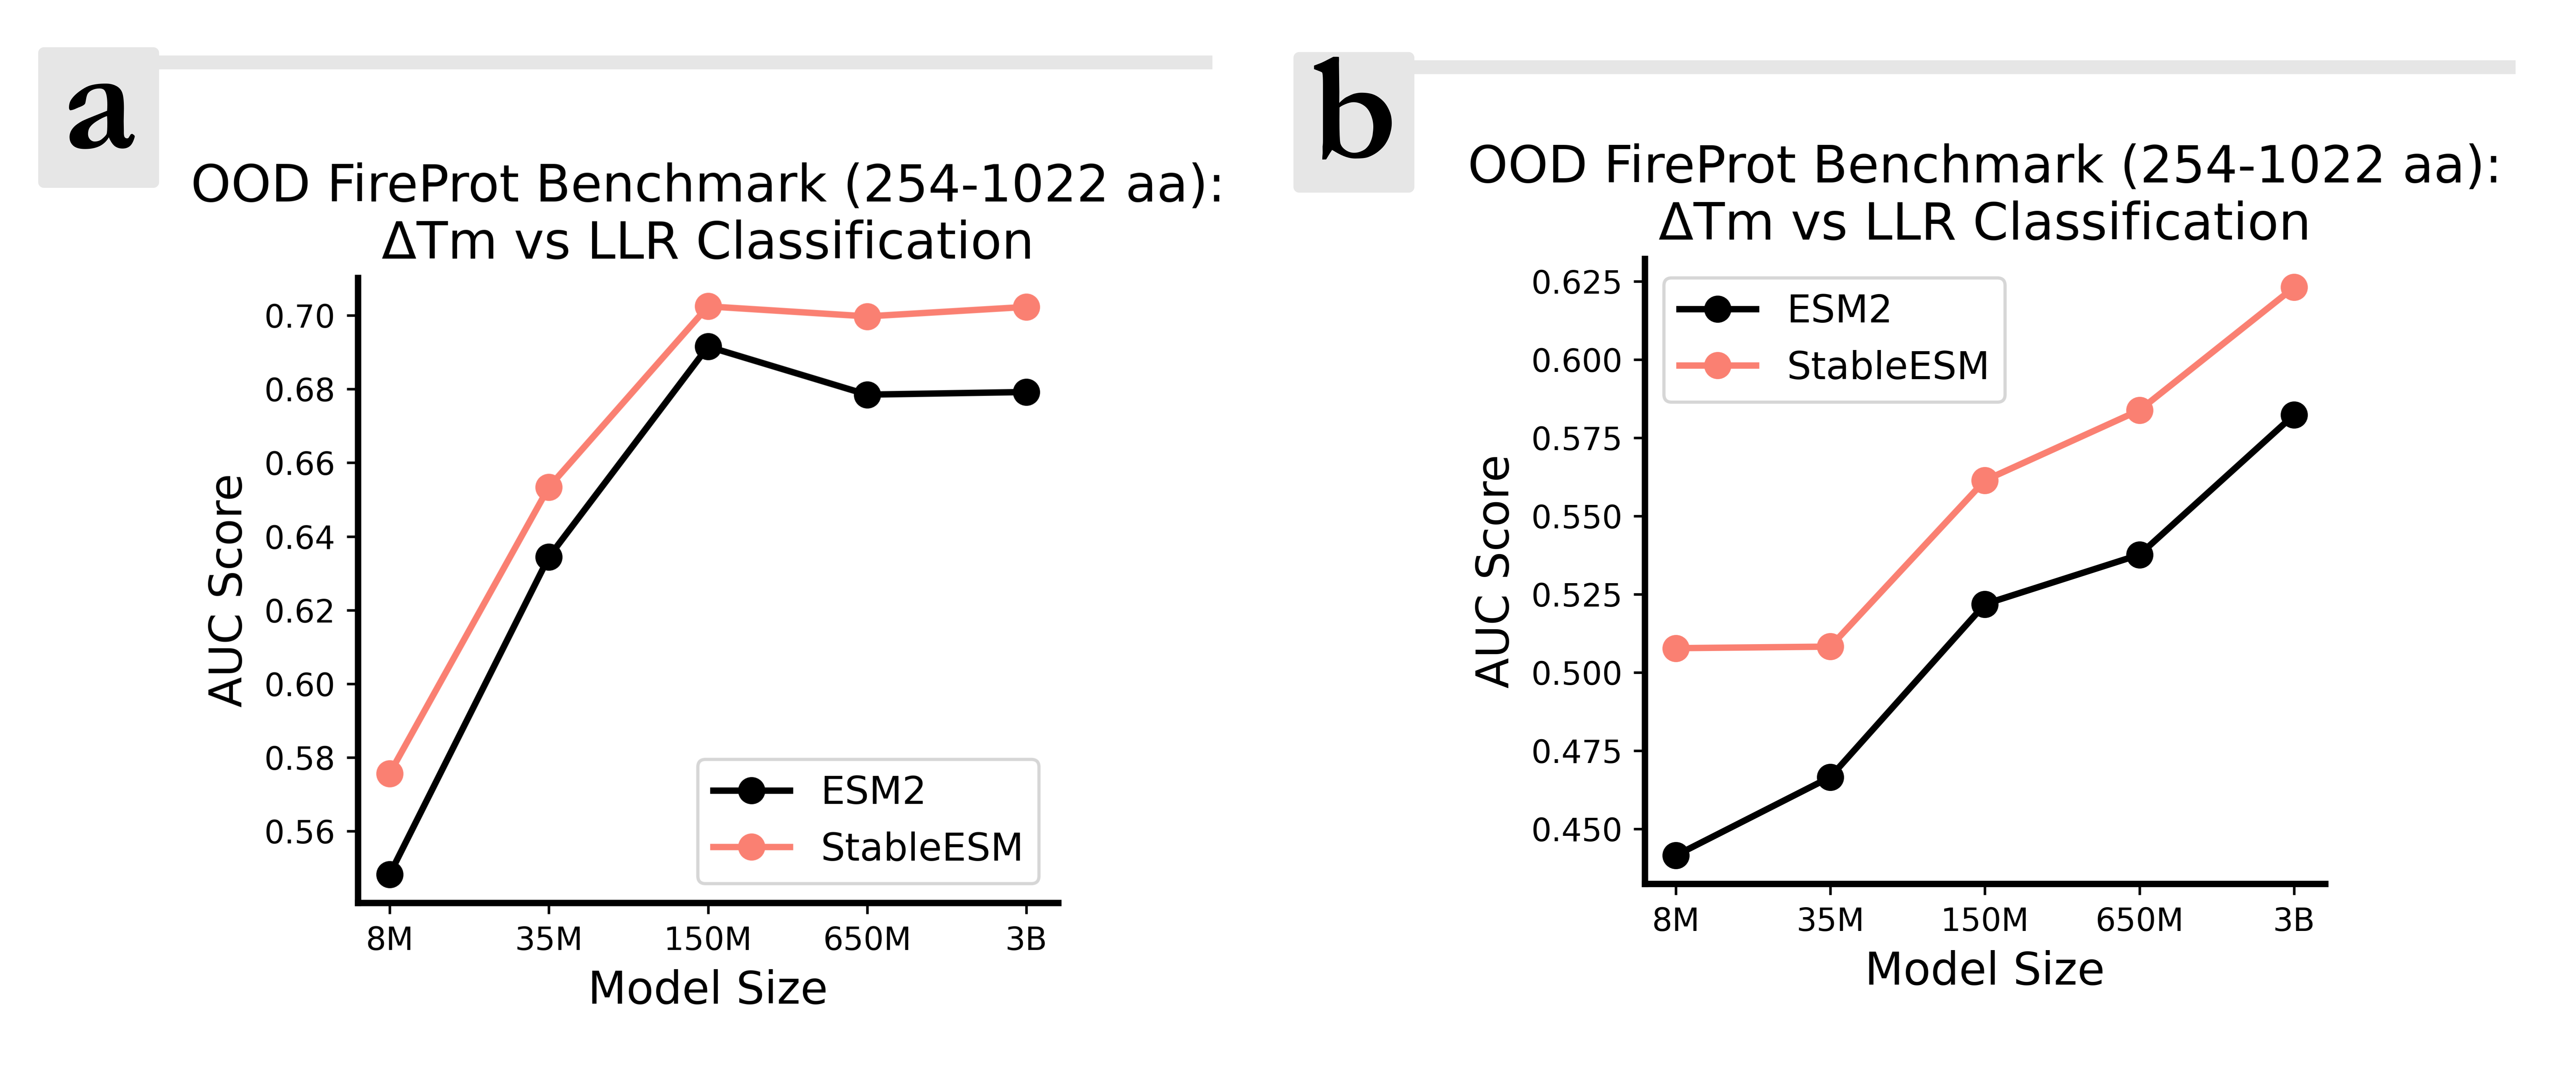
\includegraphics[width=1.0\linewidth]{figures/extended_figures/Figure_Extended5.png}
    \caption{\textbf{StableESM demonstrates improved classification performance on out-of-distribution (OOD) FireProt benchmark proteins (254-1022 amino acids).} \textbf{(a,b)} Area under the curve (AUC) scores for classifying stabilizing versus destabilizing mutations using $\Delta T_m$ measurements on completely held-out protein domains. StableESM (red) consistently outperforms ESM2 (black) across all model sizes, with performance improvements ranging from  $\sim$0.01 AUC units at smaller scales to  $\sim$0.05 AUC units at 3B parameters. While ESM2 performance plateaus at larger model sizes, StableESM continues to benefit from increased scale, achieving AUC scores of 0.71 and 0.625, respectively. These results complement the Spearman correlation analysis in Figure~\ref{fig:train_eval_stableesm}e, demonstrating that preference alignment not only improves zero-shot mutant effect prediction performance but also enhances binary classification of mutation effects on out-of-distribution protein domains, suggesting that preference alignment improves on better classifying gain-of-stability and deleterious effects.}
    \label{fig: eval_classification_on_valid_holdout}
\end{figure}


\begin{figure}[h!]
    \centering
    \includegraphics[width=1.0\linewidth]{figures/extended_figures/Figure_Extended6_final.png}
    \caption{\textbf{Preference alignment enables StableESM to generalize to out-of-distribution protein domains with improved mutational effect prediction.} \textbf{(a)} Distribution of Spearman correlation improvements (StableESM - ESM2) at 3B parameters for FireProtDB protein domains (224-1022 amino acids,$\geq$30 mutations per domain). StableESM significantly outperforms ESM2 on this out-of-distribution set (Wilcoxon signed-rank test: W = 145, p = 0.000191), with 94\% of domains showing improved rank correlation.\textbf{(b)} Model scaling analysis for the domain with largest improvement: Tyrosine-protein kinase Fyn (UniProt: P06241, 537 amino acids). StableESM 3B achieves exceptional correlation ($\rho$ = 0.886) compared to ESM2 models across all scales, demonstrating that preference alignment on shorter sequences ($\leq$224 amino acids during training) generalizes to substantially longer, unseen proteins. \textbf{(b)} Experimental validation showing relationship between $\Delta T_m$ measurements and StableESM 3B log-likelihood ratios for Tyrosine-protein kinase Fyn, with AlphaFold structure representation (grey). These results demonstrate that preference alignment enables robust generalization beyond the length distribution encountered during training, achieving strong predictive performance on completely out-of-distribution protein domains.}
    \label{fig: generalize_OOD_fireprot_StableESM}
\end{figure}


\begin{figure}[h!]
    \centering
    \includegraphics[width=1.0\linewidth]{figures/extended_figures/Figure_Extended7_final.png}
 \caption{\textbf{Preference alignment of StableESM improves binary classification of mutational effects on out-of-distribution set.} \textbf{(a)} AUC difference between StableESM and ESM2 at 3B parameters for protein domains with lengths between 224 and 1022 amino acids from the FireProtDB dataset. Only domains with $\geq$30 mutations were included to ensure robust AUC calculations. A Wilcoxon signed-rank test confirmed that StableESM significantly improves binary classification performance on the out-of-distribution (OOD) set (p $<$ 0.001). Additionally, 64.7\% of domains showed improved AUC scores. \textbf{(b)} Analysis of the domain with substantial improvement: Polyubiquitin (UniProt: P0CG63), which showed an AUC difference of 0.128 for the 3B model. This protein has a length of 381 amino acids, substantially longer than any sequence seen during preference alignment (maximum 224 amino acids), demonstrating that preference alignment on a large corpus of stability mutations can generalize to longer, unseen proteins. The progression from ESM2 (8M) at 0.333 AUC to StableESM (3B) at 0.609 AUC illustrates consistent improvement with model scale and alignment. \textbf{(c)} Relationship between experimental $\Delta\Delta G$ values and log-likelihood ratio scores from StableESM (3B) for Polyubiquitin, with AlphaFold structure representation (grey). A cubic polynomial fit (red line, $R^2$ = 0.2160) shows the model's ability to distinguish between stabilizing (negative $\Delta\Delta G$) and destabilizing (positive $\Delta\Delta G$) mutations, with the downward arrow ($\downarrow$) indicating that negative $\Delta\Delta G$ values correspond to increased protein stability.}
    \label{fig: generalize_auc_OOD_fireprot_StableESM}
\end{figure}






\clearpage
\newpage

\section{Methods}
\subsection{Curating the Stable Mutate Preference Dataset}\label{sec:dataset_curation}
\subsection{Implementing StableESM: LoRA-based Direct Preference Optimization of ESM2}\label{sec:stableesm_implementation}
\subsection{Training StableESM across model sizes using Direct Preference Optimization}\label{sec:dpo_training}
\subsection{Zero-shot mutation effect prediction using log-likelihood ratio}\label{sec:llr_prediction}
\subsection{Benchmarking StableESM on single mutations}\label{sec:single_mutation_benchmark}
\subsection{Benchmarking StableESM on double mutations}\label{sec:double_mutation_benchmark}
\subsection{Benchmarking StableESM on disorder region prediction}\label{sec:disorder_prediction}
\subsection{Testing catastrophic forgetting on structure prediction}\label{sec:structure_forgetting}
To assess whether StableESM exhibits catastrophic forgetting of structural information relative to ESM, we evaluated its learned representations using the structure module of ESMFold. Specifically, embeddings and attention maps extracted from StableESM were passed directly into the ESMFold structure module trained for 270k update steps, following the evaluation protocol used in the original ESMFold study. We evaluated models with 8M, 35M, 150M, 650M, and 3B parameters. For each model size, embeddings and attention tensors were extracted consistently with the representations used in the original ESMFold. These representations were provided as input to the ESMFold structure module, which was kept frozen throughout all experiments. No recycling steps were performed during structure prediction. Structural predictions were generated for protein targets from the CAMEO, CASP14, CASP15, and CASP16 benchmark datasets. Model performance was quantified using average per sequence pLDDT scores. 

To compare StableESM against conventional finetuning with a task-specific predictor head, we additionally evaluated representations from ESMTherm models. ESMTherm models were trained using the original ESMTherm training code and datasets and employ supervised finetuning with an explicit stability predictor head. We evaluated ESMTherm models with matching parameter sizes and extracted embeddings and attention tensors from the same attentions and representations as done for ESM and StableESM. This enabled a controlled comparison of how DPO-based optimization versus predictor head finetuning affects retention of structural signal in learned representations.

\subsection{Testing catastrophic forgetting on clinical variant prediction}\label{sec:clinical_forgetting}
\subsection{Testing catastrophic forgetting on ProteinGym benchmarks}\label{sec:proteingym_forgetting}
To further assess catastrophic forgetting in a functional prediction setting, we benchmarked StableESM representations on protein fitness prediction using the ProteinGym benchmark. Following the methodology introduced in ESM, fitness scores were computed using a log-likelihood ratio (LLR)–based metric derived from masked language modeling probabilities.

We evaluated ESM, StableESM, and ESMTherm models with 8M, 35M, 150M, 650M, and 3B parameters. For each model, predicted fitness scores were compared against experimentally measured fitness values across ProteinGym protein mutant datasets. Performance was quantified using Spearman’s rank correlation coefficient (ρ), computed separately for each dataset.

\subsection{Designing multicopper oxidase alleles and variants with StableESM}\label{sec:oxidase_design}
\subsection{Predicting mutational effects with physics-based methods: Rosetta}\label{sec:rosetta_methods}
\subsection{Experimental protocol for protein purification}\label{sec:protein_purification}
\subsection{Experimental protocol for activity assays}\label{sec:activity_assays}

\end{document}
